\documentclass[twoside]{book}

% Packages required by doxygen
\usepackage{fixltx2e}
\usepackage{calc}
\usepackage{doxygen}
\usepackage[export]{adjustbox} % also loads graphicx
\usepackage{graphicx}
\usepackage[utf8]{inputenc}
\usepackage{makeidx}
\usepackage{multicol}
\usepackage{multirow}
\PassOptionsToPackage{warn}{textcomp}
\usepackage{textcomp}
\usepackage[nointegrals]{wasysym}
\usepackage[table]{xcolor}

% Font selection
\usepackage[T1]{fontenc}
\usepackage[scaled=.90]{helvet}
\usepackage{courier}
\usepackage{amssymb}
\usepackage{sectsty}
\renewcommand{\familydefault}{\sfdefault}
\allsectionsfont{%
  \fontseries{bc}\selectfont%
  \color{darkgray}%
}
\renewcommand{\DoxyLabelFont}{%
  \fontseries{bc}\selectfont%
  \color{darkgray}%
}
\newcommand{\+}{\discretionary{\mbox{\scriptsize$\hookleftarrow$}}{}{}}

% Page & text layout
\usepackage{geometry}
\geometry{%
  a4paper,%
  top=2.5cm,%
  bottom=2.5cm,%
  left=2.5cm,%
  right=2.5cm%
}
\tolerance=750
\hfuzz=15pt
\hbadness=750
\setlength{\emergencystretch}{15pt}
\setlength{\parindent}{0cm}
\setlength{\parskip}{3ex plus 2ex minus 2ex}
\makeatletter
\renewcommand{\paragraph}{%
  \@startsection{paragraph}{4}{0ex}{-1.0ex}{1.0ex}{%
    \normalfont\normalsize\bfseries\SS@parafont%
  }%
}
\renewcommand{\subparagraph}{%
  \@startsection{subparagraph}{5}{0ex}{-1.0ex}{1.0ex}{%
    \normalfont\normalsize\bfseries\SS@subparafont%
  }%
}
\makeatother

% Headers & footers
\usepackage{fancyhdr}
\pagestyle{fancyplain}
\fancyhead[LE]{\fancyplain{}{\bfseries\thepage}}
\fancyhead[CE]{\fancyplain{}{}}
\fancyhead[RE]{\fancyplain{}{\bfseries\leftmark}}
\fancyhead[LO]{\fancyplain{}{\bfseries\rightmark}}
\fancyhead[CO]{\fancyplain{}{}}
\fancyhead[RO]{\fancyplain{}{\bfseries\thepage}}
\fancyfoot[LE]{\fancyplain{}{}}
\fancyfoot[CE]{\fancyplain{}{}}
\fancyfoot[RE]{\fancyplain{}{\bfseries\scriptsize Generated by Doxygen }}
\fancyfoot[LO]{\fancyplain{}{\bfseries\scriptsize Generated by Doxygen }}
\fancyfoot[CO]{\fancyplain{}{}}
\fancyfoot[RO]{\fancyplain{}{}}
\renewcommand{\footrulewidth}{0.4pt}
\renewcommand{\chaptermark}[1]{%
  \markboth{#1}{}%
}
\renewcommand{\sectionmark}[1]{%
  \markright{\thesection\ #1}%
}

% Indices & bibliography
\usepackage{natbib}
\usepackage[titles]{tocloft}
\setcounter{tocdepth}{3}
\setcounter{secnumdepth}{5}
\makeindex

% Hyperlinks (required, but should be loaded last)
\usepackage{ifpdf}
\ifpdf
  \usepackage[pdftex,pagebackref=true]{hyperref}
\else
  \usepackage[ps2pdf,pagebackref=true]{hyperref}
\fi
\hypersetup{%
  colorlinks=true,%
  linkcolor=blue,%
  citecolor=blue,%
  unicode%
}

% Custom commands
\newcommand{\clearemptydoublepage}{%
  \newpage{\pagestyle{empty}\cleardoublepage}%
}

\usepackage{caption}
\captionsetup{labelsep=space,justification=centering,font={bf},singlelinecheck=off,skip=4pt,position=top}

%===== C O N T E N T S =====

\begin{document}

% Titlepage & ToC
\hypersetup{pageanchor=false,
             bookmarksnumbered=true,
             pdfencoding=unicode
            }
\pagenumbering{alph}
\begin{titlepage}
\vspace*{7cm}
\begin{center}%
{\Large Slight\+C\+SV }\\
\vspace*{1cm}
{\large Generated by Doxygen 1.8.13}\\
\end{center}
\end{titlepage}
\clearemptydoublepage
\pagenumbering{roman}
\tableofcontents
\clearemptydoublepage
\pagenumbering{arabic}
\hypersetup{pageanchor=true}

%--- Begin generated contents ---
\chapter{Introduction}
\label{index}\hypertarget{index}{}Slight\+C\+SV is a C\+SV parser library written in C++. Its main purpose is to facilitate the programmatic processing of C\+SV files.

\subsection*{Features}


\begin{DoxyItemize}
\item Customizable delimiter and escape characters.
\item Flexible character manipulation capabilities (stripping, replacement).
\item Automatic handling of mac\+OS, Linux and Windows line endings.
\item Query methods for getting cell, row and column data with automatic type conversion capabilities.
\item Able to load large files ($>$ 1 GB) in reasonable time.
\item Custom exception classes inheriting from std\+::exception.
\end{DoxyItemize}

\subsection*{In addition}


\begin{DoxyItemize}
\item Detailed documentation (Doxygen).
\item Automated unit and integration testing (Cpp\+U\+Test, gcov, lcov).
\item Example code.
\end{DoxyItemize}

\section*{Getting started}

\subsection*{Operation}

After constructing the Slight\+C\+SV object (and before loading data from C\+SV file), parameters need to be set up through Slight\+C\+SV\textquotesingle{}s setter methods. File loading and processing doesn\textquotesingle{}t happen until triggering data loading through the A\+PI. If a mandatory parameter is not set, an exception will be thrown. After loading finished, data is accessible through data getter methods. Data may be unloaded later and the object can be resetted to its initial state. However, this is not mandatory as the library is only using dynamic memory with appropriate release technique (R\+A\+II).

\subsection*{Dependencies}

Slight\+C\+SV has no external dependencies. However, the following tools are used in the build pipeline to support build management, code quality and documentation.


\begin{DoxyItemize}
\item C\+Make.
\item Cpp\+U\+Test.
\item gcov, lcov.
\item Doxygen.
\end{DoxyItemize}

It is recommended to install those missing before proceeding.

\subsection*{Platform}

At the present time, the development platform is Linux. While it is possible to build and use the library on Windows, various stages of the build pipeline might fail because of missing headers and/or libraries (namely automated testing, documentation generation and code coverage report generation).

\subsection*{Project structure}

The structure inside the project root directory is as follows.


\begin{DoxyItemize}
\item bin\+: demo application build output.
\item build\+: build directory.
\item doc\+: Doxygen configuration and output.
\item inc\+: public header output (in subdirectory slightcsv).
\item lib\+: shared library output directory.
\item src\+: library and demo application sources.
\item test\+: unit and integration tests.
\end{DoxyItemize}

In order to use the pre-\/built shared library, you just need the public header (\hyperlink{slightcsv_8hpp_source}{slightcsv.\+hpp}) from inc and the library (libslightcsv.\+so or libslightcsv.\+dll on Windows) from lib.

\subsection*{Configuration and building}

For building the library from source\+:


\begin{DoxyItemize}
\item Have dependencies installed and available in the environment.
\item Edit C\+Make config file (C\+Make\+Lists.\+txt) in test and set Cpp\+U\+Test path variables.
\item Run \char`\"{}cmake .. -\/\+D\+C\+M\+A\+K\+E\+\_\+\+B\+U\+I\+L\+D\+\_\+\+T\+Y\+P\+E=\+D\+E\+B\+U\+G\char`\"{} or \char`\"{}cmake .. -\/\+D\+C\+M\+A\+K\+E\+\_\+\+B\+U\+I\+L\+D\+\_\+\+T\+Y\+P\+E=\+R\+E\+L\+E\+A\+S\+E\char`\"{} in build directory for C\+Make to generate build configuration files. In D\+E\+B\+UG, the library is built with debug symbols included while in R\+E\+L\+E\+A\+SE, those are not present (R\+E\+L\+E\+A\+SE builds use compiler optimization as well).
\item Run \char`\"{}make clean\char`\"{} in build directory to cleanup.
\item Run \char`\"{}make\char`\"{} in build directory to build the library. After issuing the command, artifacts are built and/or run in the following order\+: Slight\+C\+SV build, tests build, tests run, demo build. At the end of each stage, output files are placed in their respective directories (shared library file in lib, public header file in inc/slightcsv and executable demo application in bin).
\item Install sections are commented out in C\+Make\textquotesingle{}s config files. If you would like to use \char`\"{}make install\char`\"{}, uncomment those rows and set target paths according to your preference.
\item Documentation may be generated by issuing command \char`\"{}make docs\char`\"{}. Documentation is generated into the doc folder.
\item Code coverage report may be generated by issuing command \char`\"{}make codecov\char`\"{}. Report index file can be found at\+: build/src/\+C\+Make\+Files/slightcsv.\+dir/codecov/index.html.
\end{DoxyItemize}

\subsection*{Usage}

After including the public header in your project, you can start with the following simple example. For additional methods and parameters, please refer to the Doxygen documentation located in the doc folder.


\begin{DoxyCode}
\textcolor{preprocessor}{#include "slightcsv.hpp"}
\textcolor{preprocessor}{#include <iostream>}
\textcolor{preprocessor}{#include <string>}
\textcolor{preprocessor}{#include <vector>}

\textcolor{keyword}{using} std::cout;
\textcolor{keyword}{using} std::endl;
\textcolor{keyword}{using} std::string;
\textcolor{keyword}{using} std::vector;
\textcolor{keyword}{using} std::set;
\textcolor{keyword}{using} std::pair;
\textcolor{keyword}{using} std::map;
\textcolor{keyword}{using} \hyperlink{classutils_1_1SlightCSV}{utils::SlightCSV};

\textcolor{keywordtype}{int} main(\textcolor{keywordtype}{int} argc, \textcolor{keywordtype}{char} *argv[]) \{

    \textcolor{comment}{// construct object}
    SlightCSV scsv;

    \textcolor{comment}{// set filename}
    scsv.\hyperlink{classutils_1_1SlightCSV_a9567504e450440a9564053c8ab6f6ff9}{setFileName}(\textcolor{stringliteral}{"../test/env\_data.csv"});
    \textcolor{comment}{// set delimiter character (semicolon)}
    scsv.setSeparator(\textcolor{charliteral}{';'});
    \textcolor{comment}{// set escape character (double quote)}
    scsv.setEscape(\textcolor{charliteral}{'\(\backslash\)"'});
    \textcolor{comment}{// set characters to be stripped (stip spaces and underscores)}
    set<char> to\_strip;
    to\_strip.insert(\textcolor{charliteral}{' '});
    to\_strip.insert(\textcolor{charliteral}{'\_'});
    scsv.setStripChars(to\_strip);
    \textcolor{comment}{// set characters to be replaced (replace 'a' with 'b' and 'c' with 'd')}
    map<char, char> to\_replace;
    pair<char, char> to\_replace1(\textcolor{charliteral}{'a'}, \textcolor{charliteral}{'b'});
    pair<char, char> to\_replace2(\textcolor{charliteral}{'c'}, \textcolor{charliteral}{'d'});
    to\_replace.insert(to\_replace1);
    to\_replace.insert(to\_replace2);
    scsv.setReplaceChars(to\_replace);

    \textcolor{comment}{// load data}
    scsv.loadData();

    \textcolor{comment}{// output entity counts}
    cout << \textcolor{stringliteral}{"File contains "} << scsv.getColumnCount() << \textcolor{stringliteral}{" columns."} << endl;
    cout << \textcolor{stringliteral}{"File contains "} << scsv.getRowCount() << \textcolor{stringliteral}{" rows."} << endl;
    cout << \textcolor{stringliteral}{"Header count: "} << scsv.getHeaderCount() << \textcolor{stringliteral}{" rows."} << endl;

    \textcolor{comment}{// output row 501 (at index 500)}
    vector<string> row;
    scsv.getRow(row, 500);
    cout << \textcolor{stringliteral}{"Row 501 is: "} << endl;
    \textcolor{keywordflow}{for} (vector<string>::iterator it = row.begin(); it != row.end(); ++it) \{
        cout << *it << \textcolor{stringliteral}{" "};
    \}

    \textcolor{comment}{// output column 22 (at index 21)}
    vector<string> column;
    scsv.getColumn(column, 21);
    cout << \textcolor{stringliteral}{"Column 22 is: "} << endl;
    \textcolor{keywordflow}{for} (vector<string>::iterator it = column.begin(); it != column.end(); ++it) \{
        cout << *it << endl;
    \}

    \textcolor{comment}{// reset object to initial state (before reuse, e.g. loading another file)}
    scsv.reset();

\}
\end{DoxyCode}


\section*{Future development}

Features to be implemented in the future\+:


\begin{DoxyItemize}
\item C++11 compliant multithreading for even faster processing
\item support for U\+T\+F-\/8 character encoding
\item Extended transformation and conversion support for rows and columns
\end{DoxyItemize}

Ideas, contributions, issues and comments are welcome! 
\chapter{Namespace Index}
\section{Namespace List}
Here is a list of all documented namespaces with brief descriptions\+:\begin{DoxyCompactList}
\item\contentsline{section}{\hyperlink{namespaceutils}{utils} \\*The namespace used by all \hyperlink{classutils_1_1SlightCSV}{Slight\+C\+SV} classes and methods }{\pageref{namespaceutils}}{}
\end{DoxyCompactList}

\chapter{Hierarchical Index}
\section{Class Hierarchy}
This inheritance list is sorted roughly, but not completely, alphabetically\+:\begin{DoxyCompactList}
\item \contentsline{section}{utils\+:\+:Slight\+C\+SV}{\pageref{classutils_1_1SlightCSV}}{}
\item \contentsline{section}{utils\+:\+:Slight\+C\+S\+V\+Private}{\pageref{classutils_1_1SlightCSVPrivate}}{}
\item \contentsline{section}{utils\+:\+:Slight\+Matrix}{\pageref{classutils_1_1SlightMatrix}}{}
\item \contentsline{section}{utils\+:\+:Slight\+Row}{\pageref{classutils_1_1SlightRow}}{}
\item exception\begin{DoxyCompactList}
\item \contentsline{section}{utils\+:\+:slightcsv\+\_\+error}{\pageref{classutils_1_1slightcsv__error}}{}
\begin{DoxyCompactList}
\item \contentsline{section}{utils\+:\+:slightcsv\+\_\+data\+\_\+error}{\pageref{classutils_1_1slightcsv__data__error}}{}
\item \contentsline{section}{utils\+:\+:slightcsv\+\_\+escape\+\_\+error}{\pageref{classutils_1_1slightcsv__escape__error}}{}
\item \contentsline{section}{utils\+:\+:slightcsv\+\_\+filename\+\_\+error}{\pageref{classutils_1_1slightcsv__filename__error}}{}
\item \contentsline{section}{utils\+:\+:slightcsv\+\_\+format\+\_\+cellcnt\+\_\+error}{\pageref{classutils_1_1slightcsv__format__cellcnt__error}}{}
\item \contentsline{section}{utils\+:\+:slightcsv\+\_\+format\+\_\+header\+\_\+error}{\pageref{classutils_1_1slightcsv__format__header__error}}{}
\item \contentsline{section}{utils\+:\+:slightcsv\+\_\+index\+\_\+error}{\pageref{classutils_1_1slightcsv__index__error}}{}
\item \contentsline{section}{utils\+:\+:slightcsv\+\_\+read\+\_\+error}{\pageref{classutils_1_1slightcsv__read__error}}{}
\item \contentsline{section}{utils\+:\+:slightcsv\+\_\+replace\+\_\+error}{\pageref{classutils_1_1slightcsv__replace__error}}{}
\item \contentsline{section}{utils\+:\+:slightcsv\+\_\+separator\+\_\+error}{\pageref{classutils_1_1slightcsv__separator__error}}{}
\item \contentsline{section}{utils\+:\+:slightcsv\+\_\+strip\+\_\+error}{\pageref{classutils_1_1slightcsv__strip__error}}{}
\end{DoxyCompactList}
\item \contentsline{section}{utils\+:\+:slightmatrix\+\_\+error}{\pageref{classutils_1_1slightmatrix__error}}{}
\begin{DoxyCompactList}
\item \contentsline{section}{utils\+:\+:slightmatrix\+\_\+column\+\_\+error}{\pageref{classutils_1_1slightmatrix__column__error}}{}
\item \contentsline{section}{utils\+:\+:slightmatrix\+\_\+matrix\+\_\+error}{\pageref{classutils_1_1slightmatrix__matrix__error}}{}
\item \contentsline{section}{utils\+:\+:slightmatrix\+\_\+parameter\+\_\+error}{\pageref{classutils_1_1slightmatrix__parameter__error}}{}
\item \contentsline{section}{utils\+:\+:slightmatrix\+\_\+row\+\_\+error}{\pageref{classutils_1_1slightmatrix__row__error}}{}
\end{DoxyCompactList}
\item \contentsline{section}{utils\+:\+:slightrow\+\_\+error}{\pageref{classutils_1_1slightrow__error}}{}
\begin{DoxyCompactList}
\item \contentsline{section}{utils\+:\+:slightrow\+\_\+escape\+\_\+error}{\pageref{classutils_1_1slightrow__escape__error}}{}
\item \contentsline{section}{utils\+:\+:slightrow\+\_\+input\+\_\+error}{\pageref{classutils_1_1slightrow__input__error}}{}
\item \contentsline{section}{utils\+:\+:slightrow\+\_\+process\+\_\+error}{\pageref{classutils_1_1slightrow__process__error}}{}
\item \contentsline{section}{utils\+:\+:slightrow\+\_\+separator\+\_\+error}{\pageref{classutils_1_1slightrow__separator__error}}{}
\end{DoxyCompactList}
\end{DoxyCompactList}
\end{DoxyCompactList}

\chapter{Class Index}
\section{Class List}
Here are the classes, structs, unions and interfaces with brief descriptions\+:\begin{DoxyCompactList}
\item\contentsline{section}{\hyperlink{classutils_1_1SlightCSV}{utils\+::\+Slight\+C\+SV} }{\pageref{classutils_1_1SlightCSV}}{}
\item\contentsline{section}{\hyperlink{classutils_1_1slightcsv__data__error}{utils\+::slightcsv\+\_\+data\+\_\+error} }{\pageref{classutils_1_1slightcsv__data__error}}{}
\item\contentsline{section}{\hyperlink{classutils_1_1slightcsv__error}{utils\+::slightcsv\+\_\+error} \\*Base exception of the class (never gets thrown). Inheriting from std\+::exception }{\pageref{classutils_1_1slightcsv__error}}{}
\item\contentsline{section}{\hyperlink{classutils_1_1slightcsv__escape__error}{utils\+::slightcsv\+\_\+escape\+\_\+error} }{\pageref{classutils_1_1slightcsv__escape__error}}{}
\item\contentsline{section}{\hyperlink{classutils_1_1slightcsv__filename__error}{utils\+::slightcsv\+\_\+filename\+\_\+error} }{\pageref{classutils_1_1slightcsv__filename__error}}{}
\item\contentsline{section}{\hyperlink{classutils_1_1slightcsv__format__cellcnt__error}{utils\+::slightcsv\+\_\+format\+\_\+cellcnt\+\_\+error} }{\pageref{classutils_1_1slightcsv__format__cellcnt__error}}{}
\item\contentsline{section}{\hyperlink{classutils_1_1slightcsv__format__header__error}{utils\+::slightcsv\+\_\+format\+\_\+header\+\_\+error} }{\pageref{classutils_1_1slightcsv__format__header__error}}{}
\item\contentsline{section}{\hyperlink{classutils_1_1slightcsv__index__error}{utils\+::slightcsv\+\_\+index\+\_\+error} }{\pageref{classutils_1_1slightcsv__index__error}}{}
\item\contentsline{section}{\hyperlink{classutils_1_1slightcsv__read__error}{utils\+::slightcsv\+\_\+read\+\_\+error} }{\pageref{classutils_1_1slightcsv__read__error}}{}
\item\contentsline{section}{\hyperlink{classutils_1_1slightcsv__replace__error}{utils\+::slightcsv\+\_\+replace\+\_\+error} }{\pageref{classutils_1_1slightcsv__replace__error}}{}
\item\contentsline{section}{\hyperlink{classutils_1_1slightcsv__separator__error}{utils\+::slightcsv\+\_\+separator\+\_\+error} }{\pageref{classutils_1_1slightcsv__separator__error}}{}
\item\contentsline{section}{\hyperlink{classutils_1_1slightcsv__strip__error}{utils\+::slightcsv\+\_\+strip\+\_\+error} }{\pageref{classutils_1_1slightcsv__strip__error}}{}
\item\contentsline{section}{\hyperlink{classutils_1_1SlightCSVPrivate}{utils\+::\+Slight\+C\+S\+V\+Private} }{\pageref{classutils_1_1SlightCSVPrivate}}{}
\item\contentsline{section}{\hyperlink{classutils_1_1SlightMatrix}{utils\+::\+Slight\+Matrix} }{\pageref{classutils_1_1SlightMatrix}}{}
\item\contentsline{section}{\hyperlink{classutils_1_1slightmatrix__column__error}{utils\+::slightmatrix\+\_\+column\+\_\+error} }{\pageref{classutils_1_1slightmatrix__column__error}}{}
\item\contentsline{section}{\hyperlink{classutils_1_1slightmatrix__error}{utils\+::slightmatrix\+\_\+error} \\*Base exception of the class (never gets thrown). Inheriting from std\+::exception }{\pageref{classutils_1_1slightmatrix__error}}{}
\item\contentsline{section}{\hyperlink{classutils_1_1slightmatrix__matrix__error}{utils\+::slightmatrix\+\_\+matrix\+\_\+error} }{\pageref{classutils_1_1slightmatrix__matrix__error}}{}
\item\contentsline{section}{\hyperlink{classutils_1_1slightmatrix__parameter__error}{utils\+::slightmatrix\+\_\+parameter\+\_\+error} }{\pageref{classutils_1_1slightmatrix__parameter__error}}{}
\item\contentsline{section}{\hyperlink{classutils_1_1slightmatrix__row__error}{utils\+::slightmatrix\+\_\+row\+\_\+error} }{\pageref{classutils_1_1slightmatrix__row__error}}{}
\item\contentsline{section}{\hyperlink{classutils_1_1SlightRow}{utils\+::\+Slight\+Row} \\*The row class of the library. It is processing extracted line strings into cells }{\pageref{classutils_1_1SlightRow}}{}
\item\contentsline{section}{\hyperlink{classutils_1_1slightrow__error}{utils\+::slightrow\+\_\+error} \\*Base exception of the class (never gets thrown). Inheriting from std\+::exception }{\pageref{classutils_1_1slightrow__error}}{}
\item\contentsline{section}{\hyperlink{classutils_1_1slightrow__escape__error}{utils\+::slightrow\+\_\+escape\+\_\+error} }{\pageref{classutils_1_1slightrow__escape__error}}{}
\item\contentsline{section}{\hyperlink{classutils_1_1slightrow__input__error}{utils\+::slightrow\+\_\+input\+\_\+error} }{\pageref{classutils_1_1slightrow__input__error}}{}
\item\contentsline{section}{\hyperlink{classutils_1_1slightrow__process__error}{utils\+::slightrow\+\_\+process\+\_\+error} }{\pageref{classutils_1_1slightrow__process__error}}{}
\item\contentsline{section}{\hyperlink{classutils_1_1slightrow__separator__error}{utils\+::slightrow\+\_\+separator\+\_\+error} }{\pageref{classutils_1_1slightrow__separator__error}}{}
\end{DoxyCompactList}

\chapter{Namespace Documentation}
\hypertarget{namespaceutils}{}\section{utils Namespace Reference}
\label{namespaceutils}\index{utils@{utils}}


The namespace used by all \hyperlink{classutils_1_1SlightCSV}{Slight\+C\+SV} classes and methods.  


\subsection*{Classes}
\begin{DoxyCompactItemize}
\item 
class \hyperlink{classutils_1_1SlightCSV}{Slight\+C\+SV}
\item 
class \hyperlink{classutils_1_1slightcsv__data__error}{slightcsv\+\_\+data\+\_\+error}
\item 
class \hyperlink{classutils_1_1slightcsv__error}{slightcsv\+\_\+error}
\begin{DoxyCompactList}\small\item\em Base exception of the class (never gets thrown). Inheriting from std\+::exception. \end{DoxyCompactList}\item 
class \hyperlink{classutils_1_1slightcsv__escape__error}{slightcsv\+\_\+escape\+\_\+error}
\item 
class \hyperlink{classutils_1_1slightcsv__filename__error}{slightcsv\+\_\+filename\+\_\+error}
\item 
class \hyperlink{classutils_1_1slightcsv__format__cellcnt__error}{slightcsv\+\_\+format\+\_\+cellcnt\+\_\+error}
\item 
class \hyperlink{classutils_1_1slightcsv__format__header__error}{slightcsv\+\_\+format\+\_\+header\+\_\+error}
\item 
class \hyperlink{classutils_1_1slightcsv__index__error}{slightcsv\+\_\+index\+\_\+error}
\item 
class \hyperlink{classutils_1_1slightcsv__read__error}{slightcsv\+\_\+read\+\_\+error}
\item 
class \hyperlink{classutils_1_1slightcsv__replace__error}{slightcsv\+\_\+replace\+\_\+error}
\item 
class \hyperlink{classutils_1_1slightcsv__separator__error}{slightcsv\+\_\+separator\+\_\+error}
\item 
class \hyperlink{classutils_1_1slightcsv__strip__error}{slightcsv\+\_\+strip\+\_\+error}
\item 
class \hyperlink{classutils_1_1SlightCSVPrivate}{Slight\+C\+S\+V\+Private}
\item 
class \hyperlink{classutils_1_1SlightMatrix}{Slight\+Matrix}
\item 
class \hyperlink{classutils_1_1slightmatrix__column__error}{slightmatrix\+\_\+column\+\_\+error}
\item 
class \hyperlink{classutils_1_1slightmatrix__error}{slightmatrix\+\_\+error}
\begin{DoxyCompactList}\small\item\em Base exception of the class (never gets thrown). Inheriting from std\+::exception. \end{DoxyCompactList}\item 
class \hyperlink{classutils_1_1slightmatrix__matrix__error}{slightmatrix\+\_\+matrix\+\_\+error}
\item 
class \hyperlink{classutils_1_1slightmatrix__parameter__error}{slightmatrix\+\_\+parameter\+\_\+error}
\item 
class \hyperlink{classutils_1_1slightmatrix__row__error}{slightmatrix\+\_\+row\+\_\+error}
\item 
class \hyperlink{classutils_1_1SlightRow}{Slight\+Row}
\begin{DoxyCompactList}\small\item\em The row class of the library. It is processing extracted line strings into cells. \end{DoxyCompactList}\item 
class \hyperlink{classutils_1_1slightrow__error}{slightrow\+\_\+error}
\begin{DoxyCompactList}\small\item\em Base exception of the class (never gets thrown). Inheriting from std\+::exception. \end{DoxyCompactList}\item 
class \hyperlink{classutils_1_1slightrow__escape__error}{slightrow\+\_\+escape\+\_\+error}
\item 
class \hyperlink{classutils_1_1slightrow__input__error}{slightrow\+\_\+input\+\_\+error}
\item 
class \hyperlink{classutils_1_1slightrow__process__error}{slightrow\+\_\+process\+\_\+error}
\item 
class \hyperlink{classutils_1_1slightrow__separator__error}{slightrow\+\_\+separator\+\_\+error}
\end{DoxyCompactItemize}


\subsection{Detailed Description}
The namespace used by all \hyperlink{classutils_1_1SlightCSV}{Slight\+C\+SV} classes and methods. 
\chapter{Class Documentation}
\hypertarget{classutils_1_1SlightCSV}{}\section{utils\+:\+:Slight\+C\+SV Class Reference}
\label{classutils_1_1SlightCSV}\index{utils\+::\+Slight\+C\+SV@{utils\+::\+Slight\+C\+SV}}


{\ttfamily \#include $<$slightcsv.\+hpp$>$}

\subsection*{Public Member Functions}
\begin{DoxyCompactItemize}
\item 
\mbox{\Hypertarget{classutils_1_1SlightCSV_a9f30e030dd5eff9f7df564c9cd7a81e8}\label{classutils_1_1SlightCSV_a9f30e030dd5eff9f7df564c9cd7a81e8}} 
\hyperlink{classutils_1_1SlightCSV_a9f30e030dd5eff9f7df564c9cd7a81e8}{Slight\+C\+SV} (void)
\begin{DoxyCompactList}\small\item\em The class\textquotesingle{}s default constructor. Takes care of allocating memory for the class\textquotesingle{}s private data members. \end{DoxyCompactList}\item 
\mbox{\Hypertarget{classutils_1_1SlightCSV_abeb9790f681d93c6f8a8ba210678565b}\label{classutils_1_1SlightCSV_abeb9790f681d93c6f8a8ba210678565b}} 
\hyperlink{classutils_1_1SlightCSV_abeb9790f681d93c6f8a8ba210678565b}{$\sim$\+Slight\+C\+SV} (void)
\begin{DoxyCompactList}\small\item\em The class\textquotesingle{}s default destructor. Takes care of de-\/allocating memory held by the class\textquotesingle{}s private data members. \end{DoxyCompactList}\item 
void \hyperlink{classutils_1_1SlightCSV_a9567504e450440a9564053c8ab6f6ff9}{set\+File\+Name} (string t\+\_\+filename)
\item 
string \hyperlink{classutils_1_1SlightCSV_ad689937346e0d6dd37597e7c3458e164}{get\+File\+Name} (void) const
\item 
void \hyperlink{classutils_1_1SlightCSV_ab8cb026f9b404ef76e62eae60aecb999}{set\+Separator} (char t\+\_\+separator)
\item 
char \hyperlink{classutils_1_1SlightCSV_a72cb5e6333d648ef09fdf556d7baf15e}{get\+Separator} (void) const
\item 
void \hyperlink{classutils_1_1SlightCSV_a6673b7489c55fe9613f0ebd5dce19da4}{set\+Escape} (char t\+\_\+escape)
\item 
char \hyperlink{classutils_1_1SlightCSV_ab821a07daafa1ccaf8468ac485b226b0}{get\+Escape} (void) const
\item 
void \hyperlink{classutils_1_1SlightCSV_a8a1d201855747b4c1207ecef5ac1e2b5}{set\+Strip\+Chars} (set$<$ char $>$ \&t\+\_\+strip\+\_\+chars)
\item 
void \hyperlink{classutils_1_1SlightCSV_a13d435b5e07c827f6688efa9bf4673d4}{get\+Strip\+Chars} (set$<$ char $>$ \&t\+\_\+target) const
\item 
void \hyperlink{classutils_1_1SlightCSV_a9f7c4e3d88da03440d01b926b1fc3447}{set\+Replace\+Chars} (map$<$ char, char $>$ \&t\+\_\+rep\+\_\+chars)
\item 
void \hyperlink{classutils_1_1SlightCSV_aa28076f9867ef095802adbe0d8f966fb}{get\+Replace\+Chars} (map$<$ char, char $>$ \&t\+\_\+target) const
\item 
size\+\_\+t \hyperlink{classutils_1_1SlightCSV_adea079ec76c9ee67d096f8fd39946380}{load\+Data} (void)
\item 
size\+\_\+t \hyperlink{classutils_1_1SlightCSV_a5dcd159ef127b63942bce5498beb8dae}{get\+Column\+Count} (void) const
\item 
size\+\_\+t \hyperlink{classutils_1_1SlightCSV_a5286060190553fe7eceb973bba22ae22}{get\+Row\+Count} (void) const
\item 
void \hyperlink{classutils_1_1SlightCSV_a3d704d8bbce22b1731e383db4fc96429}{set\+Header\+Count} (size\+\_\+t t\+\_\+header\+\_\+count)
\item 
size\+\_\+t \hyperlink{classutils_1_1SlightCSV_a781ae99927f2b8d704add6a2a53e0051}{get\+Header\+Count} (void) const
\item 
{\footnotesize template$<$class T $>$ }\\void \hyperlink{classutils_1_1SlightCSV_a916d9b0b7faedc7c9af20e475c4b4cb6}{get\+Cell} (T \&t\+\_\+value, size\+\_\+t t\+\_\+row\+\_\+index, size\+\_\+t t\+\_\+column\+\_\+index) const
\item 
{\footnotesize template$<$class T $>$ }\\void \hyperlink{classutils_1_1SlightCSV_a56b9814d42283eb075bcfe3a9ca887e7}{get\+Column} (vector$<$ T $>$ \&t\+\_\+target\+\_\+column, size\+\_\+t t\+\_\+column\+\_\+index) const
\item 
{\footnotesize template$<$class T $>$ }\\void \hyperlink{classutils_1_1SlightCSV_a31db986196c89fa8b5b4f119fe548b0b}{get\+Column} (vector$<$ T $>$ \&t\+\_\+target\+\_\+column, size\+\_\+t t\+\_\+column\+\_\+index, size\+\_\+t t\+\_\+start\+\_\+cell\+\_\+index) const
\item 
{\footnotesize template$<$class T $>$ }\\void \hyperlink{classutils_1_1SlightCSV_a153cbb5059533c2103ec7ade57e4e414}{get\+Column} (vector$<$ T $>$ \&t\+\_\+target\+\_\+column, size\+\_\+t t\+\_\+column\+\_\+index, size\+\_\+t t\+\_\+start\+\_\+cell\+\_\+index, size\+\_\+t t\+\_\+cell\+\_\+count) const
\item 
void \hyperlink{classutils_1_1SlightCSV_ad4b0243488827303cd22d5efd41d96b6}{get\+Row} (vector$<$ string $>$ \&t\+\_\+target\+\_\+row, size\+\_\+t t\+\_\+row\+\_\+index) const
\item 
void \hyperlink{classutils_1_1SlightCSV_ad57a5c42bc8de6afa3d4324e52f20e2c}{get\+Row} (vector$<$ string $>$ \&t\+\_\+target\+\_\+row, size\+\_\+t t\+\_\+row\+\_\+index, size\+\_\+t t\+\_\+start\+\_\+cell\+\_\+index) const
\item 
void \hyperlink{classutils_1_1SlightCSV_a7527573dea0d6e5dc5dcfd4eab005a2b}{get\+Row} (vector$<$ string $>$ \&t\+\_\+target\+\_\+row, size\+\_\+t t\+\_\+row\+\_\+index, size\+\_\+t t\+\_\+start\+\_\+cell\+\_\+index, size\+\_\+t t\+\_\+cell\+\_\+count) const
\item 
void \hyperlink{classutils_1_1SlightCSV_aaa9c8042d6231660cb08ada7c1a8dccb}{unload\+Data} (void)
\item 
void \hyperlink{classutils_1_1SlightCSV_abc28f1e33cc67dd5d4380254070ecf97}{reset} (void)
\end{DoxyCompactItemize}


\subsection{Detailed Description}
The \char`\"{}main\char`\"{} class of the library. Provides methods for setting up the library, triggering data processing and getting the results. 

\subsection{Member Function Documentation}
\mbox{\Hypertarget{classutils_1_1SlightCSV_a916d9b0b7faedc7c9af20e475c4b4cb6}\label{classutils_1_1SlightCSV_a916d9b0b7faedc7c9af20e475c4b4cb6}} 
\index{utils\+::\+Slight\+C\+SV@{utils\+::\+Slight\+C\+SV}!get\+Cell@{get\+Cell}}
\index{get\+Cell@{get\+Cell}!utils\+::\+Slight\+C\+SV@{utils\+::\+Slight\+C\+SV}}
\subsubsection{\texorpdfstring{get\+Cell()}{getCell()}}
{\footnotesize\ttfamily template$<$class T $>$ \\
template void utils\+::\+Slight\+C\+S\+V\+::get\+Cell (\begin{DoxyParamCaption}\item[{T \&}]{t\+\_\+value,  }\item[{size\+\_\+t}]{t\+\_\+row\+\_\+index,  }\item[{size\+\_\+t}]{t\+\_\+column\+\_\+index }\end{DoxyParamCaption}) const}

Method to get the contents of a specific cell. The internal data structure stores cell values as strings. When using the method, the library tries to convert the string contents to the type supplied as the first parameter of the method. Supported types\+: int, float, double, string. If conversion fails, the value returned will be 0. In this case, it is always possible to get the value as string. 
\begin{DoxyParams}{Parameters}
{\em t\+\_\+value} & variable to hold the value of the cell. \\
\hline
{\em t\+\_\+row\+\_\+index} & index (starting from 0) of the row the cell queried. \\
\hline
{\em t\+\_\+column\+\_\+index} & index (starting from 0) of the column holding the cell queried. \\
\hline
\end{DoxyParams}
\begin{DoxySeeAlso}{See also}
\hyperlink{classutils_1_1SlightCSV_ad4b0243488827303cd22d5efd41d96b6}{get\+Row()} 

\hyperlink{classutils_1_1SlightCSV_a56b9814d42283eb075bcfe3a9ca887e7}{get\+Column()} 
\end{DoxySeeAlso}
\mbox{\Hypertarget{classutils_1_1SlightCSV_a56b9814d42283eb075bcfe3a9ca887e7}\label{classutils_1_1SlightCSV_a56b9814d42283eb075bcfe3a9ca887e7}} 
\index{utils\+::\+Slight\+C\+SV@{utils\+::\+Slight\+C\+SV}!get\+Column@{get\+Column}}
\index{get\+Column@{get\+Column}!utils\+::\+Slight\+C\+SV@{utils\+::\+Slight\+C\+SV}}
\subsubsection{\texorpdfstring{get\+Column()}{getColumn()}\hspace{0.1cm}{\footnotesize\ttfamily [1/3]}}
{\footnotesize\ttfamily template$<$class T $>$ \\
void utils\+::\+Slight\+C\+S\+V\+::get\+Column (\begin{DoxyParamCaption}\item[{vector$<$ T $>$ \&}]{t\+\_\+target\+\_\+column,  }\item[{size\+\_\+t}]{t\+\_\+column\+\_\+index }\end{DoxyParamCaption}) const}

Method to get the cells of a specific column. The column is represented in the form of a vector. The internal data structure stores cell values as strings. When using the method, the library tries to convert the string contents to the type held by the vector supplied as the method. Supported types\+: int, float, double, string. If conversion fails, the value returned will be 0. In this case, it is always possible to get the value as string. 
\begin{DoxyParams}{Parameters}
{\em t\+\_\+target\+\_\+column} & vector to hold the values of the cells in the column. \\
\hline
{\em t\+\_\+column\+\_\+index} & index (starting from 0) of the column to be returned. \\
\hline
\end{DoxyParams}
\begin{DoxySeeAlso}{See also}
\hyperlink{classutils_1_1SlightCSV_ad4b0243488827303cd22d5efd41d96b6}{get\+Row()} 

\hyperlink{classutils_1_1SlightCSV_a916d9b0b7faedc7c9af20e475c4b4cb6}{get\+Cell()} 
\end{DoxySeeAlso}
\mbox{\Hypertarget{classutils_1_1SlightCSV_a31db986196c89fa8b5b4f119fe548b0b}\label{classutils_1_1SlightCSV_a31db986196c89fa8b5b4f119fe548b0b}} 
\index{utils\+::\+Slight\+C\+SV@{utils\+::\+Slight\+C\+SV}!get\+Column@{get\+Column}}
\index{get\+Column@{get\+Column}!utils\+::\+Slight\+C\+SV@{utils\+::\+Slight\+C\+SV}}
\subsubsection{\texorpdfstring{get\+Column()}{getColumn()}\hspace{0.1cm}{\footnotesize\ttfamily [2/3]}}
{\footnotesize\ttfamily template$<$class T $>$ \\
void utils\+::\+Slight\+C\+S\+V\+::get\+Column (\begin{DoxyParamCaption}\item[{vector$<$ T $>$ \&}]{t\+\_\+target\+\_\+column,  }\item[{size\+\_\+t}]{t\+\_\+column\+\_\+index,  }\item[{size\+\_\+t}]{t\+\_\+start\+\_\+cell\+\_\+index }\end{DoxyParamCaption}) const}

This is an overloaded member function, provided for convenience. It differs from the above function only in what argument(s) it accepts. Method to get the cells of a specific column. The column is represented in the form of a vector. The internal data structure stores cell values as strings. When using the method, the library tries to convert the string contents to the type held by the vector supplied as the method. Supported types\+: int, float, double, string. If conversion fails, the value returned will be 0. In this case, it is always possible to get the value as string. 
\begin{DoxyParams}{Parameters}
{\em t\+\_\+target\+\_\+column} & vector to hold the values of the cells in the column. \\
\hline
{\em t\+\_\+column\+\_\+index} & index (starting from 0) of the column to be returned. \\
\hline
{\em t\+\_\+start\+\_\+cell\+\_\+index} & index (starting from 0) of the first vertical cell (filtering). \\
\hline
\end{DoxyParams}
\begin{DoxySeeAlso}{See also}
\hyperlink{classutils_1_1SlightCSV_ad4b0243488827303cd22d5efd41d96b6}{get\+Row()} 

\hyperlink{classutils_1_1SlightCSV_a916d9b0b7faedc7c9af20e475c4b4cb6}{get\+Cell()} 
\end{DoxySeeAlso}
\mbox{\Hypertarget{classutils_1_1SlightCSV_a153cbb5059533c2103ec7ade57e4e414}\label{classutils_1_1SlightCSV_a153cbb5059533c2103ec7ade57e4e414}} 
\index{utils\+::\+Slight\+C\+SV@{utils\+::\+Slight\+C\+SV}!get\+Column@{get\+Column}}
\index{get\+Column@{get\+Column}!utils\+::\+Slight\+C\+SV@{utils\+::\+Slight\+C\+SV}}
\subsubsection{\texorpdfstring{get\+Column()}{getColumn()}\hspace{0.1cm}{\footnotesize\ttfamily [3/3]}}
{\footnotesize\ttfamily template$<$class T $>$ \\
void utils\+::\+Slight\+C\+S\+V\+::get\+Column (\begin{DoxyParamCaption}\item[{vector$<$ T $>$ \&}]{t\+\_\+target\+\_\+column,  }\item[{size\+\_\+t}]{t\+\_\+column\+\_\+index,  }\item[{size\+\_\+t}]{t\+\_\+start\+\_\+cell\+\_\+index,  }\item[{size\+\_\+t}]{t\+\_\+cell\+\_\+count }\end{DoxyParamCaption}) const}

This is an overloaded member function, provided for convenience. It differs from the above function only in what argument(s) it accepts. Method to get the cells of a specific column. The column is represented in the form of a vector. The internal data structure stores cell values as strings. When using the method, the library tries to convert the string contents to the type held by the vector supplied as the method. Supported types\+: int, float, double, string. If conversion fails, the value returned will be 0. In this case, it is always possible to get the value as string. 
\begin{DoxyParams}{Parameters}
{\em t\+\_\+target\+\_\+column} & vector to hold the values of the cells in the column. \\
\hline
{\em t\+\_\+column\+\_\+index} & index (starting from 0) of the column to be returned. \\
\hline
{\em t\+\_\+start\+\_\+cell\+\_\+index} & index (starting from 0) of the first vertical cell (filtering) \\
\hline
{\em t\+\_\+cell\+\_\+count} & number of cells to return (beginning from the first vertical cell specified). \\
\hline
\end{DoxyParams}
\begin{DoxySeeAlso}{See also}
\hyperlink{classutils_1_1SlightCSV_ad4b0243488827303cd22d5efd41d96b6}{get\+Row()} 

\hyperlink{classutils_1_1SlightCSV_a916d9b0b7faedc7c9af20e475c4b4cb6}{get\+Cell()} 
\end{DoxySeeAlso}
\mbox{\Hypertarget{classutils_1_1SlightCSV_a5dcd159ef127b63942bce5498beb8dae}\label{classutils_1_1SlightCSV_a5dcd159ef127b63942bce5498beb8dae}} 
\index{utils\+::\+Slight\+C\+SV@{utils\+::\+Slight\+C\+SV}!get\+Column\+Count@{get\+Column\+Count}}
\index{get\+Column\+Count@{get\+Column\+Count}!utils\+::\+Slight\+C\+SV@{utils\+::\+Slight\+C\+SV}}
\subsubsection{\texorpdfstring{get\+Column\+Count()}{getColumnCount()}}
{\footnotesize\ttfamily size\+\_\+t utils\+::\+Slight\+C\+S\+V\+::get\+Column\+Count (\begin{DoxyParamCaption}\item[{void}]{ }\end{DoxyParamCaption}) const}

Method to get the number of columns in the parsed data structure. Data is held in memory. \begin{DoxyReturn}{Returns}
column count in the parsed data structure. 
\end{DoxyReturn}
\begin{DoxySeeAlso}{See also}
\hyperlink{classutils_1_1SlightCSV_a5286060190553fe7eceb973bba22ae22}{get\+Row\+Count()} 
\end{DoxySeeAlso}
\mbox{\Hypertarget{classutils_1_1SlightCSV_ab821a07daafa1ccaf8468ac485b226b0}\label{classutils_1_1SlightCSV_ab821a07daafa1ccaf8468ac485b226b0}} 
\index{utils\+::\+Slight\+C\+SV@{utils\+::\+Slight\+C\+SV}!get\+Escape@{get\+Escape}}
\index{get\+Escape@{get\+Escape}!utils\+::\+Slight\+C\+SV@{utils\+::\+Slight\+C\+SV}}
\subsubsection{\texorpdfstring{get\+Escape()}{getEscape()}}
{\footnotesize\ttfamily char utils\+::\+Slight\+C\+S\+V\+::get\+Escape (\begin{DoxyParamCaption}\item[{void}]{ }\end{DoxyParamCaption}) const}

Method to get the previously set escape character. \begin{DoxyReturn}{Returns}
previously set escape character. 
\end{DoxyReturn}
\begin{DoxySeeAlso}{See also}
\hyperlink{classutils_1_1SlightCSV_ab821a07daafa1ccaf8468ac485b226b0}{get\+Escape()} 
\end{DoxySeeAlso}
\mbox{\Hypertarget{classutils_1_1SlightCSV_ad689937346e0d6dd37597e7c3458e164}\label{classutils_1_1SlightCSV_ad689937346e0d6dd37597e7c3458e164}} 
\index{utils\+::\+Slight\+C\+SV@{utils\+::\+Slight\+C\+SV}!get\+File\+Name@{get\+File\+Name}}
\index{get\+File\+Name@{get\+File\+Name}!utils\+::\+Slight\+C\+SV@{utils\+::\+Slight\+C\+SV}}
\subsubsection{\texorpdfstring{get\+File\+Name()}{getFileName()}}
{\footnotesize\ttfamily string utils\+::\+Slight\+C\+S\+V\+::get\+File\+Name (\begin{DoxyParamCaption}\item[{void}]{ }\end{DoxyParamCaption}) const}

Method to get the previously set name of the C\+SV file to be parsed. \begin{DoxyReturn}{Returns}
previously set name and relative path of the file. 
\end{DoxyReturn}
\begin{DoxySeeAlso}{See also}
\hyperlink{classutils_1_1SlightCSV_a9567504e450440a9564053c8ab6f6ff9}{set\+File\+Name()} 
\end{DoxySeeAlso}
\mbox{\Hypertarget{classutils_1_1SlightCSV_a781ae99927f2b8d704add6a2a53e0051}\label{classutils_1_1SlightCSV_a781ae99927f2b8d704add6a2a53e0051}} 
\index{utils\+::\+Slight\+C\+SV@{utils\+::\+Slight\+C\+SV}!get\+Header\+Count@{get\+Header\+Count}}
\index{get\+Header\+Count@{get\+Header\+Count}!utils\+::\+Slight\+C\+SV@{utils\+::\+Slight\+C\+SV}}
\subsubsection{\texorpdfstring{get\+Header\+Count()}{getHeaderCount()}}
{\footnotesize\ttfamily size\+\_\+t utils\+::\+Slight\+C\+S\+V\+::get\+Header\+Count (\begin{DoxyParamCaption}\item[{void}]{ }\end{DoxyParamCaption}) const}

Method to get the number of header rows at the beginning of the parsed file. After loading the data it returns an automatically detected value which may be overridden by the user. \begin{DoxyReturn}{Returns}
number of header rows at the beginning of the parsed file. 
\end{DoxyReturn}
\begin{DoxySeeAlso}{See also}
\hyperlink{classutils_1_1SlightCSV_a3d704d8bbce22b1731e383db4fc96429}{set\+Header\+Count()} 
\end{DoxySeeAlso}
\mbox{\Hypertarget{classutils_1_1SlightCSV_aa28076f9867ef095802adbe0d8f966fb}\label{classutils_1_1SlightCSV_aa28076f9867ef095802adbe0d8f966fb}} 
\index{utils\+::\+Slight\+C\+SV@{utils\+::\+Slight\+C\+SV}!get\+Replace\+Chars@{get\+Replace\+Chars}}
\index{get\+Replace\+Chars@{get\+Replace\+Chars}!utils\+::\+Slight\+C\+SV@{utils\+::\+Slight\+C\+SV}}
\subsubsection{\texorpdfstring{get\+Replace\+Chars()}{getReplaceChars()}}
{\footnotesize\ttfamily void utils\+::\+Slight\+C\+S\+V\+::get\+Replace\+Chars (\begin{DoxyParamCaption}\item[{map$<$ char, char $>$ \&}]{t\+\_\+target }\end{DoxyParamCaption}) const}

Method to get the previously set map of character pair(s) to be replaced in the input of the parser. 
\begin{DoxyParams}{Parameters}
{\em t\+\_\+target} & map that gets populated with the previously defined map of character pair(s) to be replaced. \\
\hline
\end{DoxyParams}
\begin{DoxySeeAlso}{See also}
\hyperlink{classutils_1_1SlightCSV_a9f7c4e3d88da03440d01b926b1fc3447}{set\+Replace\+Chars()} 
\end{DoxySeeAlso}
\mbox{\Hypertarget{classutils_1_1SlightCSV_ad4b0243488827303cd22d5efd41d96b6}\label{classutils_1_1SlightCSV_ad4b0243488827303cd22d5efd41d96b6}} 
\index{utils\+::\+Slight\+C\+SV@{utils\+::\+Slight\+C\+SV}!get\+Row@{get\+Row}}
\index{get\+Row@{get\+Row}!utils\+::\+Slight\+C\+SV@{utils\+::\+Slight\+C\+SV}}
\subsubsection{\texorpdfstring{get\+Row()}{getRow()}\hspace{0.1cm}{\footnotesize\ttfamily [1/3]}}
{\footnotesize\ttfamily void utils\+::\+Slight\+C\+S\+V\+::get\+Row (\begin{DoxyParamCaption}\item[{vector$<$ string $>$ \&}]{t\+\_\+target\+\_\+row,  }\item[{size\+\_\+t}]{t\+\_\+row\+\_\+index }\end{DoxyParamCaption}) const}

Method to get the cells of a specific row. The row is represented in the form of a vector. The internal data structure stores cell values as strings. When using the method, the library returns cells in a row as strings. 
\begin{DoxyParams}{Parameters}
{\em t\+\_\+target\+\_\+row} & vector to hold the values of the cells in the row. \\
\hline
{\em t\+\_\+row\+\_\+index} & index (starting from 0) of the row to be returned. \\
\hline
\end{DoxyParams}
\begin{DoxySeeAlso}{See also}
\hyperlink{classutils_1_1SlightCSV_a56b9814d42283eb075bcfe3a9ca887e7}{get\+Column()} 

\hyperlink{classutils_1_1SlightCSV_a916d9b0b7faedc7c9af20e475c4b4cb6}{get\+Cell()} 
\end{DoxySeeAlso}
\mbox{\Hypertarget{classutils_1_1SlightCSV_ad57a5c42bc8de6afa3d4324e52f20e2c}\label{classutils_1_1SlightCSV_ad57a5c42bc8de6afa3d4324e52f20e2c}} 
\index{utils\+::\+Slight\+C\+SV@{utils\+::\+Slight\+C\+SV}!get\+Row@{get\+Row}}
\index{get\+Row@{get\+Row}!utils\+::\+Slight\+C\+SV@{utils\+::\+Slight\+C\+SV}}
\subsubsection{\texorpdfstring{get\+Row()}{getRow()}\hspace{0.1cm}{\footnotesize\ttfamily [2/3]}}
{\footnotesize\ttfamily void utils\+::\+Slight\+C\+S\+V\+::get\+Row (\begin{DoxyParamCaption}\item[{vector$<$ string $>$ \&}]{t\+\_\+target\+\_\+row,  }\item[{size\+\_\+t}]{t\+\_\+row\+\_\+index,  }\item[{size\+\_\+t}]{t\+\_\+start\+\_\+cell\+\_\+index }\end{DoxyParamCaption}) const}

This is an overloaded member function, provided for convenience. It differs from the above function only in what argument(s) it accepts. Method to get the cells of a specific row. The row is represented in the form of a vector. The internal data structure stores cell values as strings. When using the method, the library returns cells in a row as strings. 
\begin{DoxyParams}{Parameters}
{\em t\+\_\+target\+\_\+row} & vector to hold the values of the cells in the row. \\
\hline
{\em t\+\_\+row\+\_\+index} & index (starting from 0) of the row to be returned. \\
\hline
{\em t\+\_\+start\+\_\+cell\+\_\+index} & index (starting from 0) of the first horizontal cell (filtering). \\
\hline
\end{DoxyParams}
\begin{DoxySeeAlso}{See also}
\hyperlink{classutils_1_1SlightCSV_a56b9814d42283eb075bcfe3a9ca887e7}{get\+Column()} 

\hyperlink{classutils_1_1SlightCSV_a916d9b0b7faedc7c9af20e475c4b4cb6}{get\+Cell()} 
\end{DoxySeeAlso}
\mbox{\Hypertarget{classutils_1_1SlightCSV_a7527573dea0d6e5dc5dcfd4eab005a2b}\label{classutils_1_1SlightCSV_a7527573dea0d6e5dc5dcfd4eab005a2b}} 
\index{utils\+::\+Slight\+C\+SV@{utils\+::\+Slight\+C\+SV}!get\+Row@{get\+Row}}
\index{get\+Row@{get\+Row}!utils\+::\+Slight\+C\+SV@{utils\+::\+Slight\+C\+SV}}
\subsubsection{\texorpdfstring{get\+Row()}{getRow()}\hspace{0.1cm}{\footnotesize\ttfamily [3/3]}}
{\footnotesize\ttfamily void utils\+::\+Slight\+C\+S\+V\+::get\+Row (\begin{DoxyParamCaption}\item[{vector$<$ string $>$ \&}]{t\+\_\+target\+\_\+row,  }\item[{size\+\_\+t}]{t\+\_\+row\+\_\+index,  }\item[{size\+\_\+t}]{t\+\_\+start\+\_\+cell\+\_\+index,  }\item[{size\+\_\+t}]{t\+\_\+cell\+\_\+count }\end{DoxyParamCaption}) const}

This is an overloaded member function, provided for convenience. It differs from the above function only in what argument(s) it accepts. Method to get the cells of a specific row. The row is represented in the form of a vector. The internal data structure stores cell values as strings. When using the method, the library returns cells in a row as strings. 
\begin{DoxyParams}{Parameters}
{\em t\+\_\+target\+\_\+row} & vector to hold the values of the cells in the row. \\
\hline
{\em t\+\_\+row\+\_\+index} & index (starting from 0) of the row to be returned. \\
\hline
{\em t\+\_\+start\+\_\+cell\+\_\+index} & index (starting from 0) of the first horizontal cell (filtering). \\
\hline
{\em t\+\_\+cell\+\_\+count} & number of cells to return (beginning from the first horizontal cell specified). \\
\hline
\end{DoxyParams}
\begin{DoxySeeAlso}{See also}
\hyperlink{classutils_1_1SlightCSV_a56b9814d42283eb075bcfe3a9ca887e7}{get\+Column()} 

\hyperlink{classutils_1_1SlightCSV_a916d9b0b7faedc7c9af20e475c4b4cb6}{get\+Cell()} 
\end{DoxySeeAlso}
\mbox{\Hypertarget{classutils_1_1SlightCSV_a5286060190553fe7eceb973bba22ae22}\label{classutils_1_1SlightCSV_a5286060190553fe7eceb973bba22ae22}} 
\index{utils\+::\+Slight\+C\+SV@{utils\+::\+Slight\+C\+SV}!get\+Row\+Count@{get\+Row\+Count}}
\index{get\+Row\+Count@{get\+Row\+Count}!utils\+::\+Slight\+C\+SV@{utils\+::\+Slight\+C\+SV}}
\subsubsection{\texorpdfstring{get\+Row\+Count()}{getRowCount()}}
{\footnotesize\ttfamily size\+\_\+t utils\+::\+Slight\+C\+S\+V\+::get\+Row\+Count (\begin{DoxyParamCaption}\item[{void}]{ }\end{DoxyParamCaption}) const}

Method to get the number of rows in the parsed data structure. Data is held in memory. \begin{DoxyReturn}{Returns}
row count in the parsed data structure. 
\end{DoxyReturn}
\begin{DoxySeeAlso}{See also}
\hyperlink{classutils_1_1SlightCSV_a5dcd159ef127b63942bce5498beb8dae}{get\+Column\+Count()} 
\end{DoxySeeAlso}
\mbox{\Hypertarget{classutils_1_1SlightCSV_a72cb5e6333d648ef09fdf556d7baf15e}\label{classutils_1_1SlightCSV_a72cb5e6333d648ef09fdf556d7baf15e}} 
\index{utils\+::\+Slight\+C\+SV@{utils\+::\+Slight\+C\+SV}!get\+Separator@{get\+Separator}}
\index{get\+Separator@{get\+Separator}!utils\+::\+Slight\+C\+SV@{utils\+::\+Slight\+C\+SV}}
\subsubsection{\texorpdfstring{get\+Separator()}{getSeparator()}}
{\footnotesize\ttfamily char utils\+::\+Slight\+C\+S\+V\+::get\+Separator (\begin{DoxyParamCaption}\item[{void}]{ }\end{DoxyParamCaption}) const}

Method to get the previously set delimiter character. \begin{DoxyReturn}{Returns}
previously set delimiter character. 
\end{DoxyReturn}
\begin{DoxySeeAlso}{See also}
\hyperlink{classutils_1_1SlightCSV_ab8cb026f9b404ef76e62eae60aecb999}{set\+Separator()} 
\end{DoxySeeAlso}
\mbox{\Hypertarget{classutils_1_1SlightCSV_a13d435b5e07c827f6688efa9bf4673d4}\label{classutils_1_1SlightCSV_a13d435b5e07c827f6688efa9bf4673d4}} 
\index{utils\+::\+Slight\+C\+SV@{utils\+::\+Slight\+C\+SV}!get\+Strip\+Chars@{get\+Strip\+Chars}}
\index{get\+Strip\+Chars@{get\+Strip\+Chars}!utils\+::\+Slight\+C\+SV@{utils\+::\+Slight\+C\+SV}}
\subsubsection{\texorpdfstring{get\+Strip\+Chars()}{getStripChars()}}
{\footnotesize\ttfamily void utils\+::\+Slight\+C\+S\+V\+::get\+Strip\+Chars (\begin{DoxyParamCaption}\item[{set$<$ char $>$ \&}]{t\+\_\+target }\end{DoxyParamCaption}) const}

Method to get the previously defined set of character(s) to be stripped from the input of the parser. 
\begin{DoxyParams}{Parameters}
{\em t\+\_\+target} & set that gets populated with the previously defined set of characters to be stripped.\\
\hline
\end{DoxyParams}
\begin{DoxySeeAlso}{See also}
\hyperlink{classutils_1_1SlightCSV_a8a1d201855747b4c1207ecef5ac1e2b5}{set\+Strip\+Chars()} 
\end{DoxySeeAlso}
\mbox{\Hypertarget{classutils_1_1SlightCSV_adea079ec76c9ee67d096f8fd39946380}\label{classutils_1_1SlightCSV_adea079ec76c9ee67d096f8fd39946380}} 
\index{utils\+::\+Slight\+C\+SV@{utils\+::\+Slight\+C\+SV}!load\+Data@{load\+Data}}
\index{load\+Data@{load\+Data}!utils\+::\+Slight\+C\+SV@{utils\+::\+Slight\+C\+SV}}
\subsubsection{\texorpdfstring{load\+Data()}{loadData()}}
{\footnotesize\ttfamily size\+\_\+t utils\+::\+Slight\+C\+S\+V\+::load\+Data (\begin{DoxyParamCaption}\item[{void}]{ }\end{DoxyParamCaption})}

Method to trigger data loading. Requires filename and delimiter to be set before calling it. \begin{DoxyReturn}{Returns}
the number of records loaded. 
\end{DoxyReturn}
\begin{DoxySeeAlso}{See also}
\hyperlink{classutils_1_1SlightCSV_aaa9c8042d6231660cb08ada7c1a8dccb}{unload\+Data()} 
\end{DoxySeeAlso}
\mbox{\Hypertarget{classutils_1_1SlightCSV_abc28f1e33cc67dd5d4380254070ecf97}\label{classutils_1_1SlightCSV_abc28f1e33cc67dd5d4380254070ecf97}} 
\index{utils\+::\+Slight\+C\+SV@{utils\+::\+Slight\+C\+SV}!reset@{reset}}
\index{reset@{reset}!utils\+::\+Slight\+C\+SV@{utils\+::\+Slight\+C\+SV}}
\subsubsection{\texorpdfstring{reset()}{reset()}}
{\footnotesize\ttfamily void utils\+::\+Slight\+C\+S\+V\+::reset (\begin{DoxyParamCaption}\item[{void}]{ }\end{DoxyParamCaption})}

Method to reset the library to its initial state. Unloads any data structure loaded previously and resets settings to their initial state. Optional, library will not leak if not used. \mbox{\Hypertarget{classutils_1_1SlightCSV_a6673b7489c55fe9613f0ebd5dce19da4}\label{classutils_1_1SlightCSV_a6673b7489c55fe9613f0ebd5dce19da4}} 
\index{utils\+::\+Slight\+C\+SV@{utils\+::\+Slight\+C\+SV}!set\+Escape@{set\+Escape}}
\index{set\+Escape@{set\+Escape}!utils\+::\+Slight\+C\+SV@{utils\+::\+Slight\+C\+SV}}
\subsubsection{\texorpdfstring{set\+Escape()}{setEscape()}}
{\footnotesize\ttfamily void utils\+::\+Slight\+C\+S\+V\+::set\+Escape (\begin{DoxyParamCaption}\item[{char}]{t\+\_\+escape }\end{DoxyParamCaption})}

Method to set the escape character. It is used to escape other characters in the file to be processed. Escaped delimiter and new line characters are not processed and are propagated to processed \char`\"{}cells\char`\"{}. Setting (or not setting) the escape character not in accordance with the file format may trigger exceptions (e.\+g. cell count mismatch in row). Order of execution\+: strip, escape, replace. Characters enclosed between escape characters will be escaped even if escape characters are stripped or replaced. Method is optional. If used, set it before triggering data loading. 
\begin{DoxyParams}{Parameters}
{\em t\+\_\+escape} & character to be used to escape a group of characters in the input. \\
\hline
\end{DoxyParams}
\begin{DoxySeeAlso}{See also}
\hyperlink{classutils_1_1SlightCSV_ab821a07daafa1ccaf8468ac485b226b0}{get\+Escape()} 
\end{DoxySeeAlso}
\mbox{\Hypertarget{classutils_1_1SlightCSV_a9567504e450440a9564053c8ab6f6ff9}\label{classutils_1_1SlightCSV_a9567504e450440a9564053c8ab6f6ff9}} 
\index{utils\+::\+Slight\+C\+SV@{utils\+::\+Slight\+C\+SV}!set\+File\+Name@{set\+File\+Name}}
\index{set\+File\+Name@{set\+File\+Name}!utils\+::\+Slight\+C\+SV@{utils\+::\+Slight\+C\+SV}}
\subsubsection{\texorpdfstring{set\+File\+Name()}{setFileName()}}
{\footnotesize\ttfamily void utils\+::\+Slight\+C\+S\+V\+::set\+File\+Name (\begin{DoxyParamCaption}\item[{string}]{t\+\_\+filename }\end{DoxyParamCaption})}

Method to set the name of the C\+SV file to be parsed. Required before triggering data loading. 
\begin{DoxyParams}{Parameters}
{\em t\+\_\+filename} & name and relative path of the file. \\
\hline
\end{DoxyParams}
\begin{DoxySeeAlso}{See also}
\hyperlink{classutils_1_1SlightCSV_ad689937346e0d6dd37597e7c3458e164}{get\+File\+Name()} 
\end{DoxySeeAlso}
\mbox{\Hypertarget{classutils_1_1SlightCSV_a3d704d8bbce22b1731e383db4fc96429}\label{classutils_1_1SlightCSV_a3d704d8bbce22b1731e383db4fc96429}} 
\index{utils\+::\+Slight\+C\+SV@{utils\+::\+Slight\+C\+SV}!set\+Header\+Count@{set\+Header\+Count}}
\index{set\+Header\+Count@{set\+Header\+Count}!utils\+::\+Slight\+C\+SV@{utils\+::\+Slight\+C\+SV}}
\subsubsection{\texorpdfstring{set\+Header\+Count()}{setHeaderCount()}}
{\footnotesize\ttfamily void utils\+::\+Slight\+C\+S\+V\+::set\+Header\+Count (\begin{DoxyParamCaption}\item[{size\+\_\+t}]{t\+\_\+header\+\_\+count }\end{DoxyParamCaption})}

Method to override and set the number of header rows in the output of the parser. The library tries to detect and count header rows automatically. 
\begin{DoxyParams}{Parameters}
{\em t\+\_\+header\+\_\+count} & the number of header rows at the beginning of the C\+SV file. \\
\hline
\end{DoxyParams}
\begin{DoxySeeAlso}{See also}
\hyperlink{classutils_1_1SlightCSV_a781ae99927f2b8d704add6a2a53e0051}{get\+Header\+Count()} 
\end{DoxySeeAlso}
\mbox{\Hypertarget{classutils_1_1SlightCSV_a9f7c4e3d88da03440d01b926b1fc3447}\label{classutils_1_1SlightCSV_a9f7c4e3d88da03440d01b926b1fc3447}} 
\index{utils\+::\+Slight\+C\+SV@{utils\+::\+Slight\+C\+SV}!set\+Replace\+Chars@{set\+Replace\+Chars}}
\index{set\+Replace\+Chars@{set\+Replace\+Chars}!utils\+::\+Slight\+C\+SV@{utils\+::\+Slight\+C\+SV}}
\subsubsection{\texorpdfstring{set\+Replace\+Chars()}{setReplaceChars()}}
{\footnotesize\ttfamily void utils\+::\+Slight\+C\+S\+V\+::set\+Replace\+Chars (\begin{DoxyParamCaption}\item[{map$<$ char, char $>$ \&}]{t\+\_\+rep\+\_\+chars }\end{DoxyParamCaption})}

Method to define a map of character pair(s) to be replaced in the input of the parser. The map\textquotesingle{}s \char`\"{}key\char`\"{} character is replaced by the \char`\"{}value\char`\"{} character in the input. Order of execution\+: strip, escape, replace. Escape characters may be replaced, but characters enclosed between escape characters will be escaped and present in the output. Stripped characters won\textquotesingle{}t be seen by the method. Optional method. If used, set it before triggering data loading. 
\begin{DoxyParams}{Parameters}
{\em t\+\_\+rep\+\_\+chars} & a map of \char`\"{}replacee\char`\"{} and \char`\"{}replacer\char`\"{} characters. \\
\hline
\end{DoxyParams}
\begin{DoxySeeAlso}{See also}
\hyperlink{classutils_1_1SlightCSV_aa28076f9867ef095802adbe0d8f966fb}{get\+Replace\+Chars()} 
\end{DoxySeeAlso}
\mbox{\Hypertarget{classutils_1_1SlightCSV_ab8cb026f9b404ef76e62eae60aecb999}\label{classutils_1_1SlightCSV_ab8cb026f9b404ef76e62eae60aecb999}} 
\index{utils\+::\+Slight\+C\+SV@{utils\+::\+Slight\+C\+SV}!set\+Separator@{set\+Separator}}
\index{set\+Separator@{set\+Separator}!utils\+::\+Slight\+C\+SV@{utils\+::\+Slight\+C\+SV}}
\subsubsection{\texorpdfstring{set\+Separator()}{setSeparator()}}
{\footnotesize\ttfamily void utils\+::\+Slight\+C\+S\+V\+::set\+Separator (\begin{DoxyParamCaption}\item[{char}]{t\+\_\+separator }\end{DoxyParamCaption})}

Method to set the delimiter character. It is used as a separator between \char`\"{}cells\char`\"{} in a row. Required before triggering data loading. 
\begin{DoxyParams}{Parameters}
{\em t\+\_\+separator} & character to use as delimiter. \\
\hline
\end{DoxyParams}
\begin{DoxySeeAlso}{See also}
\hyperlink{classutils_1_1SlightCSV_a72cb5e6333d648ef09fdf556d7baf15e}{get\+Separator()} 
\end{DoxySeeAlso}
\mbox{\Hypertarget{classutils_1_1SlightCSV_a8a1d201855747b4c1207ecef5ac1e2b5}\label{classutils_1_1SlightCSV_a8a1d201855747b4c1207ecef5ac1e2b5}} 
\index{utils\+::\+Slight\+C\+SV@{utils\+::\+Slight\+C\+SV}!set\+Strip\+Chars@{set\+Strip\+Chars}}
\index{set\+Strip\+Chars@{set\+Strip\+Chars}!utils\+::\+Slight\+C\+SV@{utils\+::\+Slight\+C\+SV}}
\subsubsection{\texorpdfstring{set\+Strip\+Chars()}{setStripChars()}}
{\footnotesize\ttfamily void utils\+::\+Slight\+C\+S\+V\+::set\+Strip\+Chars (\begin{DoxyParamCaption}\item[{set$<$ char $>$ \&}]{t\+\_\+strip\+\_\+chars }\end{DoxyParamCaption})}

Method to define a set of character(s) to be stripped from the input of the parser. Order of execution\+: strip, escape, replace. Escape characters may be stripped, but characters enclosed between escape characters will be escaped and present in the output. Stripped characters won\textquotesingle{}t be seen by replace. Optional method. If used, set it before triggering data loading. 
\begin{DoxyParams}{Parameters}
{\em t\+\_\+strip\+\_\+chars} & a set of characters previously populated with characters to be stripped. \\
\hline
\end{DoxyParams}
\begin{DoxySeeAlso}{See also}
\hyperlink{classutils_1_1SlightCSV_a13d435b5e07c827f6688efa9bf4673d4}{get\+Strip\+Chars()} 
\end{DoxySeeAlso}
\mbox{\Hypertarget{classutils_1_1SlightCSV_aaa9c8042d6231660cb08ada7c1a8dccb}\label{classutils_1_1SlightCSV_aaa9c8042d6231660cb08ada7c1a8dccb}} 
\index{utils\+::\+Slight\+C\+SV@{utils\+::\+Slight\+C\+SV}!unload\+Data@{unload\+Data}}
\index{unload\+Data@{unload\+Data}!utils\+::\+Slight\+C\+SV@{utils\+::\+Slight\+C\+SV}}
\subsubsection{\texorpdfstring{unload\+Data()}{unloadData()}}
{\footnotesize\ttfamily void utils\+::\+Slight\+C\+S\+V\+::unload\+Data (\begin{DoxyParamCaption}\item[{void}]{ }\end{DoxyParamCaption})}

Method to unload data structure from memory. Settings (filename, delimiter, character manipulation settings) are preserved. Data queries cannot be made until loading a data structure. Optional, library will not leak if not used. \begin{DoxySeeAlso}{See also}
\hyperlink{classutils_1_1SlightCSV_adea079ec76c9ee67d096f8fd39946380}{load\+Data()} 
\end{DoxySeeAlso}


The documentation for this class was generated from the following files\+:\begin{DoxyCompactItemize}
\item 
/home/hsg/\+Documents/projects/slightcsv/src/slightcsv.\+hpp\item 
/home/hsg/\+Documents/projects/slightcsv/src/slightcsv.\+cpp\end{DoxyCompactItemize}

\hypertarget{classutils_1_1slightcsv__data__error}{}\section{utils\+:\+:slightcsv\+\_\+data\+\_\+error Class Reference}
\label{classutils_1_1slightcsv__data__error}\index{utils\+::slightcsv\+\_\+data\+\_\+error@{utils\+::slightcsv\+\_\+data\+\_\+error}}


{\ttfamily \#include $<$slightcsv.\+hpp$>$}



Inheritance diagram for utils\+:\+:slightcsv\+\_\+data\+\_\+error\+:
\nopagebreak
\begin{figure}[H]
\begin{center}
\leavevmode
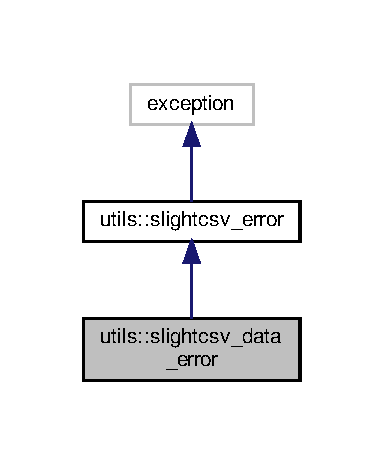
\includegraphics[width=184pt]{classutils_1_1slightcsv__data__error__inherit__graph}
\end{center}
\end{figure}


Collaboration diagram for utils\+:\+:slightcsv\+\_\+data\+\_\+error\+:
\nopagebreak
\begin{figure}[H]
\begin{center}
\leavevmode
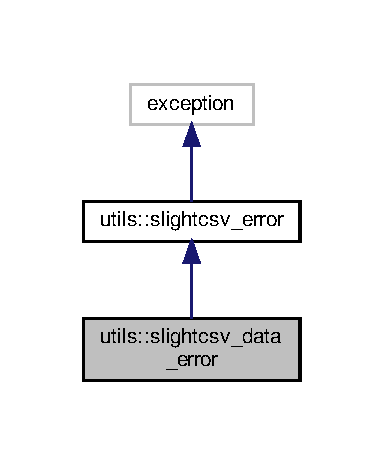
\includegraphics[width=184pt]{classutils_1_1slightcsv__data__error__coll__graph}
\end{center}
\end{figure}


\subsection{Detailed Description}
Exception inheriting from \hyperlink{classutils_1_1slightcsv__error}{slightcsv\+\_\+error}. It is thrown when\+:
\begin{DoxyItemize}
\item data query methods are called before loading a data structure 
\end{DoxyItemize}

The documentation for this class was generated from the following file\+:\begin{DoxyCompactItemize}
\item 
/home/hsg/\+Documents/projects/slightcsv/src/slightcsv.\+hpp\end{DoxyCompactItemize}

\hypertarget{classutils_1_1slightcsv__error}{}\section{utils\+:\+:slightcsv\+\_\+error Class Reference}
\label{classutils_1_1slightcsv__error}\index{utils\+::slightcsv\+\_\+error@{utils\+::slightcsv\+\_\+error}}


Base exception of the class (never gets thrown). Inheriting from std\+::exception.  




{\ttfamily \#include $<$slightcsv.\+hpp$>$}



Inheritance diagram for utils\+:\+:slightcsv\+\_\+error\+:
\nopagebreak
\begin{figure}[H]
\begin{center}
\leavevmode
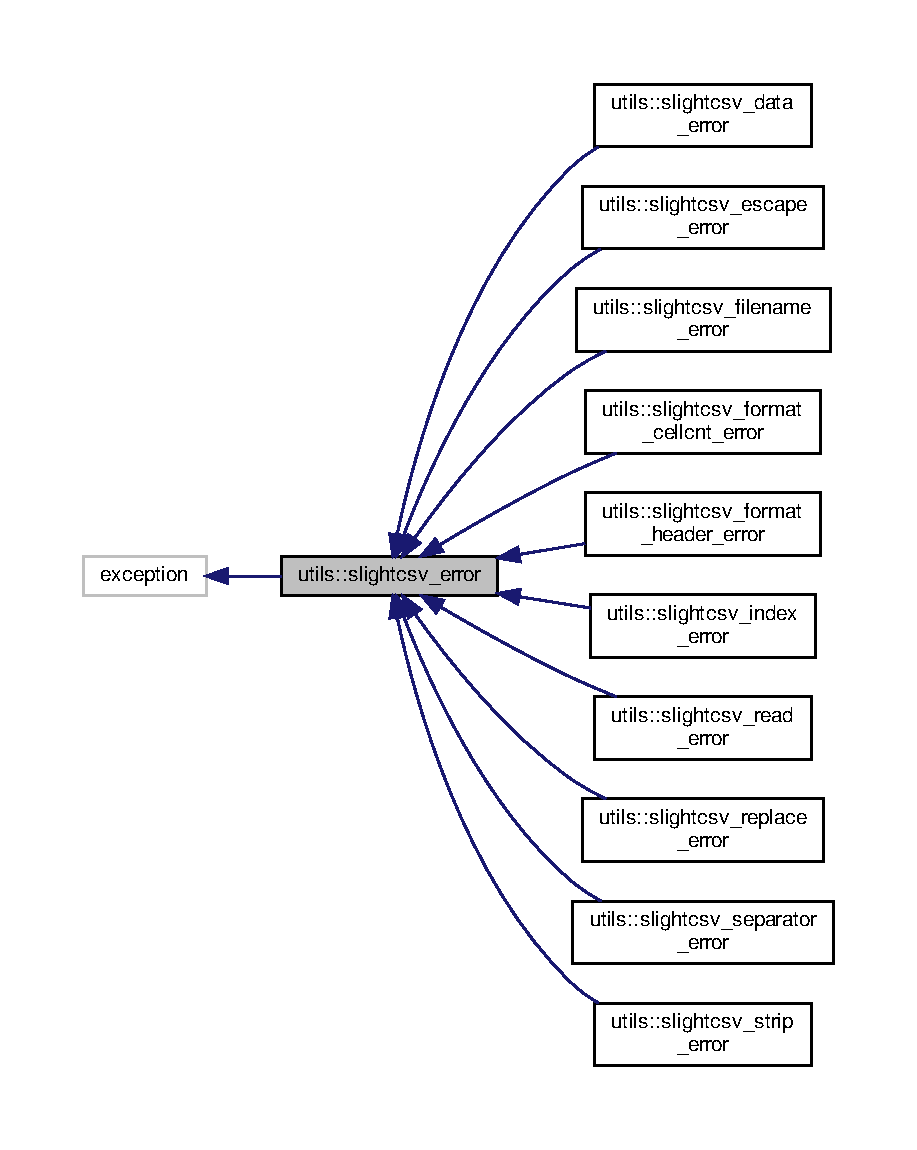
\includegraphics[width=350pt]{classutils_1_1slightcsv__error__inherit__graph}
\end{center}
\end{figure}


Collaboration diagram for utils\+:\+:slightcsv\+\_\+error\+:
\nopagebreak
\begin{figure}[H]
\begin{center}
\leavevmode
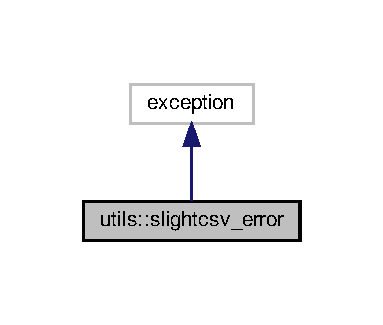
\includegraphics[width=184pt]{classutils_1_1slightcsv__error__coll__graph}
\end{center}
\end{figure}


\subsection{Detailed Description}
Base exception of the class (never gets thrown). Inheriting from std\+::exception. 

The documentation for this class was generated from the following file\+:\begin{DoxyCompactItemize}
\item 
/home/hsg/\+Documents/projects/slightcsv/src/slightcsv.\+hpp\end{DoxyCompactItemize}

\hypertarget{classutils_1_1slightcsv__escape__error}{}\section{utils\+:\+:slightcsv\+\_\+escape\+\_\+error Class Reference}
\label{classutils_1_1slightcsv__escape__error}\index{utils\+::slightcsv\+\_\+escape\+\_\+error@{utils\+::slightcsv\+\_\+escape\+\_\+error}}


{\ttfamily \#include $<$slightcsv.\+hpp$>$}



Inheritance diagram for utils\+:\+:slightcsv\+\_\+escape\+\_\+error\+:\nopagebreak
\begin{figure}[H]
\begin{center}
\leavevmode
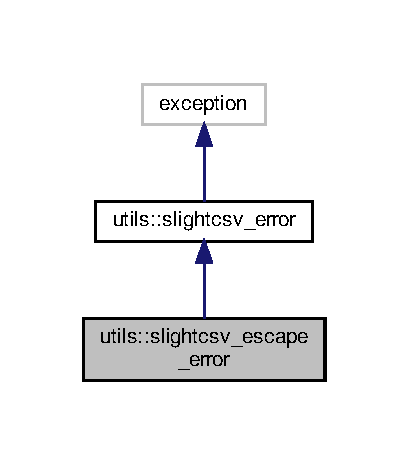
\includegraphics[width=196pt]{classutils_1_1slightcsv__escape__error__inherit__graph}
\end{center}
\end{figure}


Collaboration diagram for utils\+:\+:slightcsv\+\_\+escape\+\_\+error\+:\nopagebreak
\begin{figure}[H]
\begin{center}
\leavevmode
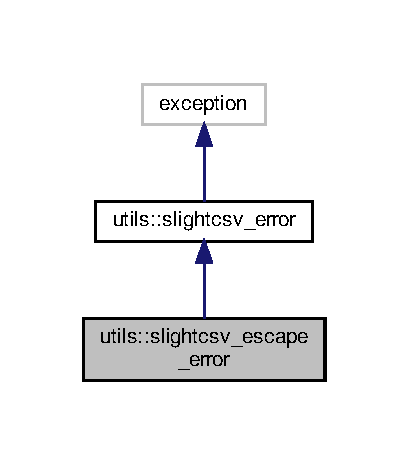
\includegraphics[width=196pt]{classutils_1_1slightcsv__escape__error__coll__graph}
\end{center}
\end{figure}


\subsection{Detailed Description}
Exception inheriting from \hyperlink{classutils_1_1slightcsv__error}{slightcsv\+\_\+error}. It is thrown when\+:
\begin{DoxyItemize}
\item queried escape character value is zero (not set)
\item trying to set escape character with zero value 
\end{DoxyItemize}

The documentation for this class was generated from the following file\+:\begin{DoxyCompactItemize}
\item 
/home/hsg/\+Documents/projects/slightcsv/src/slightcsv.\+hpp\end{DoxyCompactItemize}

\hypertarget{classutils_1_1slightcsv__filename__error}{}\section{utils\+:\+:slightcsv\+\_\+filename\+\_\+error Class Reference}
\label{classutils_1_1slightcsv__filename__error}\index{utils\+::slightcsv\+\_\+filename\+\_\+error@{utils\+::slightcsv\+\_\+filename\+\_\+error}}


{\ttfamily \#include $<$slightcsv.\+hpp$>$}



Inheritance diagram for utils\+:\+:slightcsv\+\_\+filename\+\_\+error\+:\nopagebreak
\begin{figure}[H]
\begin{center}
\leavevmode
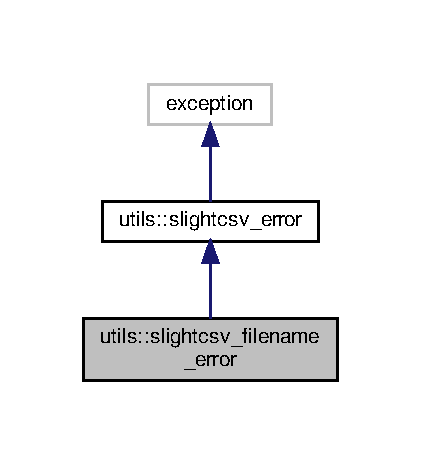
\includegraphics[width=202pt]{classutils_1_1slightcsv__filename__error__inherit__graph}
\end{center}
\end{figure}


Collaboration diagram for utils\+:\+:slightcsv\+\_\+filename\+\_\+error\+:\nopagebreak
\begin{figure}[H]
\begin{center}
\leavevmode
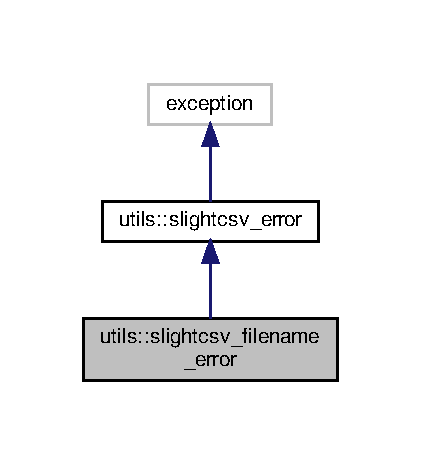
\includegraphics[width=202pt]{classutils_1_1slightcsv__filename__error__coll__graph}
\end{center}
\end{figure}


\subsection{Detailed Description}
Exception inheriting from \hyperlink{classutils_1_1slightcsv__error}{slightcsv\+\_\+error}. It is thrown when\+:
\begin{DoxyItemize}
\item data cannot be loaded (file not found)
\item queried filename is empty (not set)
\item trying to set empty filename 
\end{DoxyItemize}

The documentation for this class was generated from the following file\+:\begin{DoxyCompactItemize}
\item 
/home/hsg/\+Documents/projects/slightcsv/src/slightcsv.\+hpp\end{DoxyCompactItemize}

\hypertarget{classutils_1_1slightcsv__format__cellcnt__error}{}\section{utils\+:\+:slightcsv\+\_\+format\+\_\+cellcnt\+\_\+error Class Reference}
\label{classutils_1_1slightcsv__format__cellcnt__error}\index{utils\+::slightcsv\+\_\+format\+\_\+cellcnt\+\_\+error@{utils\+::slightcsv\+\_\+format\+\_\+cellcnt\+\_\+error}}


{\ttfamily \#include $<$slightcsv.\+hpp$>$}



Inheritance diagram for utils\+:\+:slightcsv\+\_\+format\+\_\+cellcnt\+\_\+error\+:\nopagebreak
\begin{figure}[H]
\begin{center}
\leavevmode
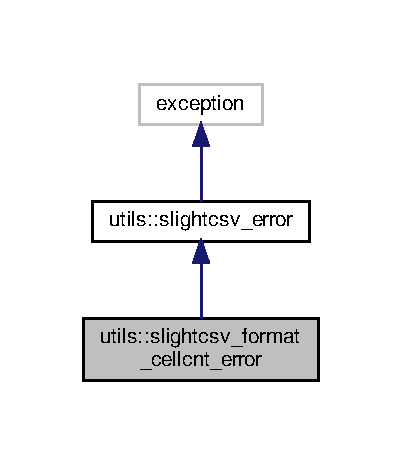
\includegraphics[width=193pt]{classutils_1_1slightcsv__format__cellcnt__error__inherit__graph}
\end{center}
\end{figure}


Collaboration diagram for utils\+:\+:slightcsv\+\_\+format\+\_\+cellcnt\+\_\+error\+:\nopagebreak
\begin{figure}[H]
\begin{center}
\leavevmode
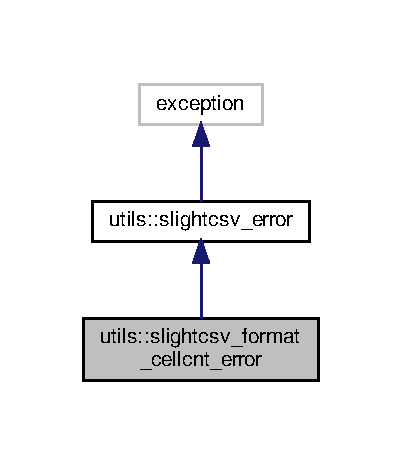
\includegraphics[width=193pt]{classutils_1_1slightcsv__format__cellcnt__error__coll__graph}
\end{center}
\end{figure}


\subsection{Detailed Description}
Exception inheriting from \hyperlink{classutils_1_1slightcsv__error}{slightcsv\+\_\+error}. It is thrown when\+:
\begin{DoxyItemize}
\item the C\+SV file format is invalid (inconsistency in terms of cell quantity in a row)
\item settings of the parser cause the C\+SV file format to seem invalid (as a consequence of character manipulation with escape, strip and replace) 
\end{DoxyItemize}

The documentation for this class was generated from the following file\+:\begin{DoxyCompactItemize}
\item 
/home/hsg/\+Documents/projects/slightcsv/src/slightcsv.\+hpp\end{DoxyCompactItemize}

\hypertarget{classutils_1_1slightcsv__format__header__error}{}\section{utils\+:\+:slightcsv\+\_\+format\+\_\+header\+\_\+error Class Reference}
\label{classutils_1_1slightcsv__format__header__error}\index{utils\+::slightcsv\+\_\+format\+\_\+header\+\_\+error@{utils\+::slightcsv\+\_\+format\+\_\+header\+\_\+error}}


{\ttfamily \#include $<$slightcsv.\+hpp$>$}



Inheritance diagram for utils\+:\+:slightcsv\+\_\+format\+\_\+header\+\_\+error\+:
\nopagebreak
\begin{figure}[H]
\begin{center}
\leavevmode
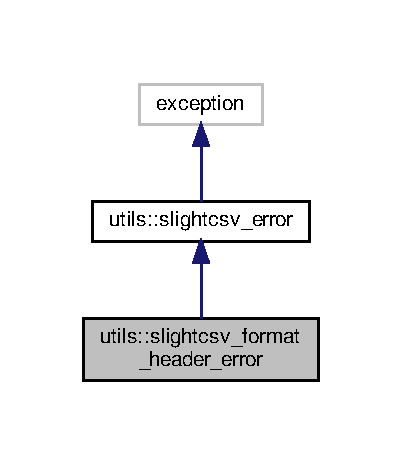
\includegraphics[width=193pt]{classutils_1_1slightcsv__format__header__error__inherit__graph}
\end{center}
\end{figure}


Collaboration diagram for utils\+:\+:slightcsv\+\_\+format\+\_\+header\+\_\+error\+:
\nopagebreak
\begin{figure}[H]
\begin{center}
\leavevmode
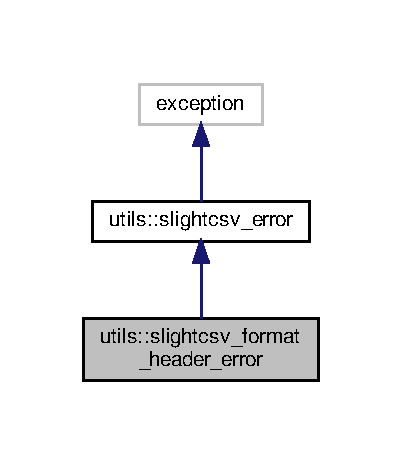
\includegraphics[width=193pt]{classutils_1_1slightcsv__format__header__error__coll__graph}
\end{center}
\end{figure}


\subsection{Detailed Description}
Exception inheriting from \hyperlink{classutils_1_1slightcsv__error}{slightcsv\+\_\+error}. It is thrown when\+:
\begin{DoxyItemize}
\item intermediate header row is found after the beginning of the file 
\end{DoxyItemize}

The documentation for this class was generated from the following file\+:\begin{DoxyCompactItemize}
\item 
/home/hsg/\+Documents/projects/slightcsv/src/slightcsv.\+hpp\end{DoxyCompactItemize}

\hypertarget{classutils_1_1slightcsv__index__error}{}\section{utils\+:\+:slightcsv\+\_\+index\+\_\+error Class Reference}
\label{classutils_1_1slightcsv__index__error}\index{utils\+::slightcsv\+\_\+index\+\_\+error@{utils\+::slightcsv\+\_\+index\+\_\+error}}


{\ttfamily \#include $<$slightcsv.\+hpp$>$}



Inheritance diagram for utils\+:\+:slightcsv\+\_\+index\+\_\+error\+:\nopagebreak
\begin{figure}[H]
\begin{center}
\leavevmode
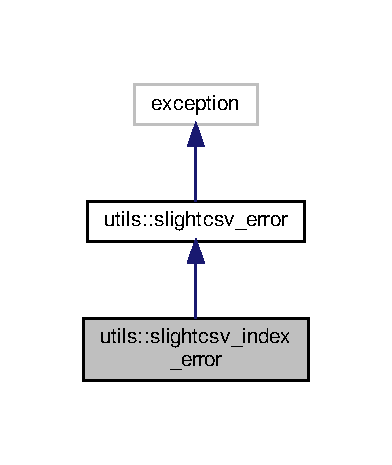
\includegraphics[width=188pt]{classutils_1_1slightcsv__index__error__inherit__graph}
\end{center}
\end{figure}


Collaboration diagram for utils\+:\+:slightcsv\+\_\+index\+\_\+error\+:\nopagebreak
\begin{figure}[H]
\begin{center}
\leavevmode
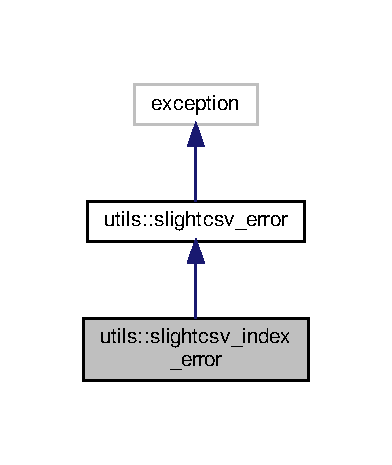
\includegraphics[width=188pt]{classutils_1_1slightcsv__index__error__coll__graph}
\end{center}
\end{figure}


\subsection{Detailed Description}
Exception inheriting from \hyperlink{classutils_1_1slightcsv__error}{slightcsv\+\_\+error}. It is thrown when\+:
\begin{DoxyItemize}
\item data query methods called with out-\/of-\/range row index
\item data query methods called with out-\/of-\/range column index 
\end{DoxyItemize}

The documentation for this class was generated from the following file\+:\begin{DoxyCompactItemize}
\item 
/home/hsg/\+Documents/projects/slightcsv/src/slightcsv.\+hpp\end{DoxyCompactItemize}

\hypertarget{classutils_1_1slightcsv__read__error}{}\section{utils\+:\+:slightcsv\+\_\+read\+\_\+error Class Reference}
\label{classutils_1_1slightcsv__read__error}\index{utils\+::slightcsv\+\_\+read\+\_\+error@{utils\+::slightcsv\+\_\+read\+\_\+error}}


{\ttfamily \#include $<$slightcsv.\+hpp$>$}



Inheritance diagram for utils\+:\+:slightcsv\+\_\+read\+\_\+error\+:\nopagebreak
\begin{figure}[H]
\begin{center}
\leavevmode
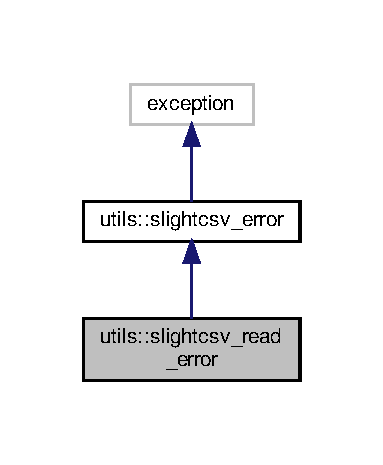
\includegraphics[width=184pt]{classutils_1_1slightcsv__read__error__inherit__graph}
\end{center}
\end{figure}


Collaboration diagram for utils\+:\+:slightcsv\+\_\+read\+\_\+error\+:\nopagebreak
\begin{figure}[H]
\begin{center}
\leavevmode
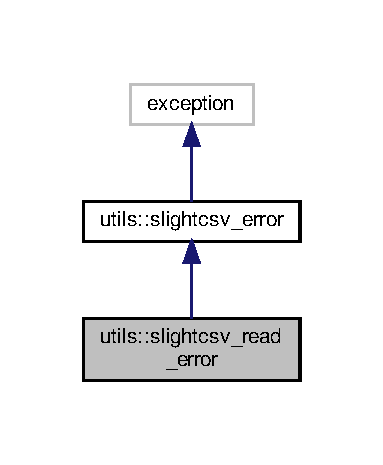
\includegraphics[width=184pt]{classutils_1_1slightcsv__read__error__coll__graph}
\end{center}
\end{figure}


\subsection{Detailed Description}
Exception inheriting from \hyperlink{classutils_1_1slightcsv__error}{slightcsv\+\_\+error}. It is thrown when\+:
\begin{DoxyItemize}
\item file read error occurred before reaching the end of file (E\+OF) 
\end{DoxyItemize}

The documentation for this class was generated from the following file\+:\begin{DoxyCompactItemize}
\item 
/home/hsg/\+Documents/projects/slightcsv/src/slightcsv.\+hpp\end{DoxyCompactItemize}

\hypertarget{classutils_1_1slightcsv__replace__error}{}\section{utils\+:\+:slightcsv\+\_\+replace\+\_\+error Class Reference}
\label{classutils_1_1slightcsv__replace__error}\index{utils\+::slightcsv\+\_\+replace\+\_\+error@{utils\+::slightcsv\+\_\+replace\+\_\+error}}


{\ttfamily \#include $<$slightcsv.\+hpp$>$}



Inheritance diagram for utils\+:\+:slightcsv\+\_\+replace\+\_\+error\+:
\nopagebreak
\begin{figure}[H]
\begin{center}
\leavevmode
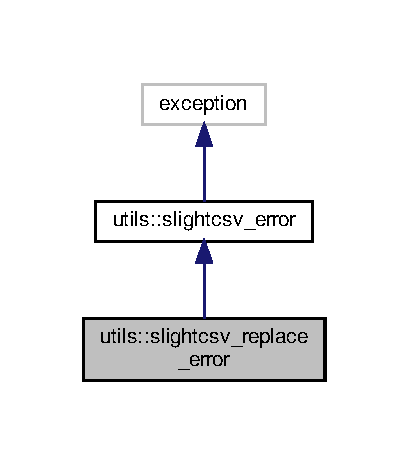
\includegraphics[width=196pt]{classutils_1_1slightcsv__replace__error__inherit__graph}
\end{center}
\end{figure}


Collaboration diagram for utils\+:\+:slightcsv\+\_\+replace\+\_\+error\+:
\nopagebreak
\begin{figure}[H]
\begin{center}
\leavevmode
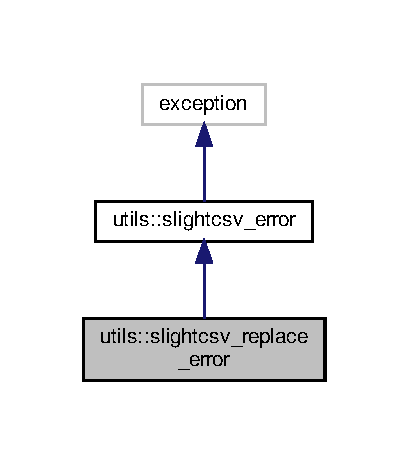
\includegraphics[width=196pt]{classutils_1_1slightcsv__replace__error__coll__graph}
\end{center}
\end{figure}


\subsection{Detailed Description}
Exception inheriting from \hyperlink{classutils_1_1slightcsv__error}{slightcsv\+\_\+error}. It is thrown when\+:
\begin{DoxyItemize}
\item queried replace character map is empty (not set)
\item trying to set empty replace character map 
\end{DoxyItemize}

The documentation for this class was generated from the following file\+:\begin{DoxyCompactItemize}
\item 
/home/hsg/\+Documents/projects/slightcsv/src/slightcsv.\+hpp\end{DoxyCompactItemize}

\hypertarget{classutils_1_1slightcsv__separator__error}{}\section{utils\+:\+:slightcsv\+\_\+separator\+\_\+error Class Reference}
\label{classutils_1_1slightcsv__separator__error}\index{utils\+::slightcsv\+\_\+separator\+\_\+error@{utils\+::slightcsv\+\_\+separator\+\_\+error}}


{\ttfamily \#include $<$slightcsv.\+hpp$>$}



Inheritance diagram for utils\+:\+:slightcsv\+\_\+separator\+\_\+error\+:
\nopagebreak
\begin{figure}[H]
\begin{center}
\leavevmode
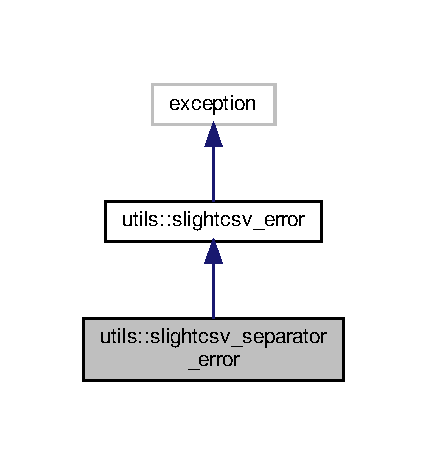
\includegraphics[width=205pt]{classutils_1_1slightcsv__separator__error__inherit__graph}
\end{center}
\end{figure}


Collaboration diagram for utils\+:\+:slightcsv\+\_\+separator\+\_\+error\+:
\nopagebreak
\begin{figure}[H]
\begin{center}
\leavevmode
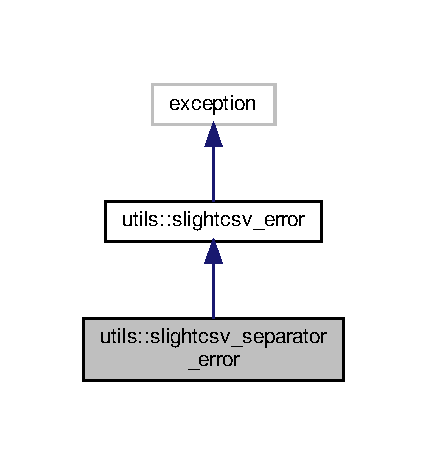
\includegraphics[width=205pt]{classutils_1_1slightcsv__separator__error__coll__graph}
\end{center}
\end{figure}


\subsection{Detailed Description}
Exception inheriting from \hyperlink{classutils_1_1slightcsv__error}{slightcsv\+\_\+error}. It is thrown when\+:
\begin{DoxyItemize}
\item queried delimiter character value is zero (not set)
\item trying to set delimiter character with zero value 
\end{DoxyItemize}

The documentation for this class was generated from the following file\+:\begin{DoxyCompactItemize}
\item 
/home/hsg/\+Documents/projects/slightcsv/src/slightcsv.\+hpp\end{DoxyCompactItemize}

\hypertarget{classutils_1_1slightcsv__strip__error}{}\section{utils\+:\+:slightcsv\+\_\+strip\+\_\+error Class Reference}
\label{classutils_1_1slightcsv__strip__error}\index{utils\+::slightcsv\+\_\+strip\+\_\+error@{utils\+::slightcsv\+\_\+strip\+\_\+error}}


{\ttfamily \#include $<$slightcsv.\+hpp$>$}



Inheritance diagram for utils\+:\+:slightcsv\+\_\+strip\+\_\+error\+:
\nopagebreak
\begin{figure}[H]
\begin{center}
\leavevmode
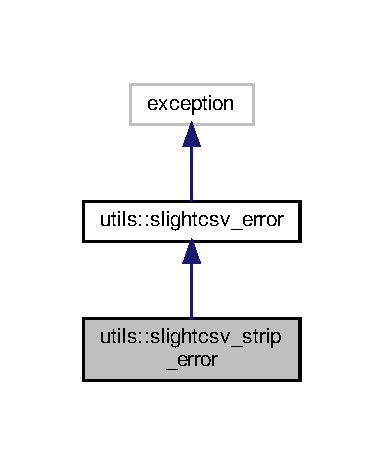
\includegraphics[width=184pt]{classutils_1_1slightcsv__strip__error__inherit__graph}
\end{center}
\end{figure}


Collaboration diagram for utils\+:\+:slightcsv\+\_\+strip\+\_\+error\+:
\nopagebreak
\begin{figure}[H]
\begin{center}
\leavevmode
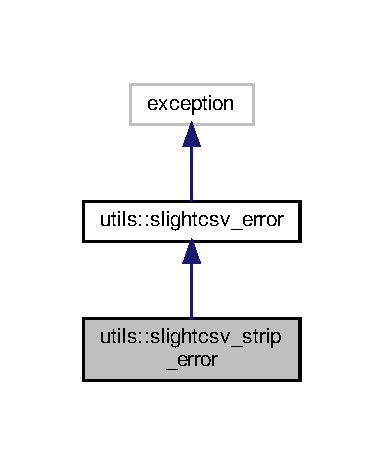
\includegraphics[width=184pt]{classutils_1_1slightcsv__strip__error__coll__graph}
\end{center}
\end{figure}


\subsection{Detailed Description}
Exception inheriting from std\+::exception. It is thrown when\+:
\begin{DoxyItemize}
\item queried strip character set is empty (not set)
\item trying to set empty strip character set 
\end{DoxyItemize}

The documentation for this class was generated from the following file\+:\begin{DoxyCompactItemize}
\item 
/home/hsg/\+Documents/projects/slightcsv/src/slightcsv.\+hpp\end{DoxyCompactItemize}

\hypertarget{classutils_1_1SlightMatrix}{}\section{utils\+:\+:Slight\+Matrix Class Reference}
\label{classutils_1_1SlightMatrix}\index{utils\+::\+Slight\+Matrix@{utils\+::\+Slight\+Matrix}}


{\ttfamily \#include $<$slightmatrix.\+hpp$>$}

\subsection*{Public Member Functions}
\begin{DoxyCompactItemize}
\item 
\mbox{\Hypertarget{classutils_1_1SlightMatrix_a2c2eb567ef914ecde524b3af725258fd}\label{classutils_1_1SlightMatrix_a2c2eb567ef914ecde524b3af725258fd}} 
\hyperlink{classutils_1_1SlightMatrix_a2c2eb567ef914ecde524b3af725258fd}{Slight\+Matrix} (void)
\begin{DoxyCompactList}\small\item\em The class\textquotesingle{}s default constructor. \end{DoxyCompactList}\item 
void \hyperlink{classutils_1_1SlightMatrix_ac0c6859041a90cfdf39d6c4f5a668814}{set\+Capacity} (const size\+\_\+t t\+\_\+cell\+\_\+count)
\item 
size\+\_\+t \hyperlink{classutils_1_1SlightMatrix_addbfd1ec641100a7cda0b4f6e39ae676}{get\+Capacity} (void) const
\item 
void \hyperlink{classutils_1_1SlightMatrix_a5f633b5225716e60a69cdca3b43f380c}{set\+Column\+Count} (const size\+\_\+t t\+\_\+column\+\_\+count)
\item 
size\+\_\+t \hyperlink{classutils_1_1SlightMatrix_aa08a3c2d096ac82b1688b1edc5bb71fd}{get\+Column\+Count} (void) const
\item 
void \hyperlink{classutils_1_1SlightMatrix_ac2d5111e5a9865886f5370bf1487d04c}{add\+Cell} (const string t\+\_\+cell)
\item 
void \hyperlink{classutils_1_1SlightMatrix_ad8874298dd54748b660fe9546ff9b332}{add\+Cells} (const vector$<$ string $>$ \&t\+\_\+cells)
\item 
void \hyperlink{classutils_1_1SlightMatrix_abe914aa8f3178afae99ec31502ba2d35}{set\+Header\+Count} (const size\+\_\+t t\+\_\+header\+\_\+count)
\item 
size\+\_\+t \hyperlink{classutils_1_1SlightMatrix_ac3ba42c47509027bd1c4a07055f347b9}{get\+Header\+Count} (void) const
\item 
bool \hyperlink{classutils_1_1SlightMatrix_a536e733a179ee3eaeb5c75986cc477d3}{validate} (void) const
\item 
size\+\_\+t \hyperlink{classutils_1_1SlightMatrix_af171e463492b423251369cd7b8799a97}{get\+Row\+Count} (void) const
\item 
{\footnotesize template$<$class T $>$ }\\void \hyperlink{classutils_1_1SlightMatrix_a38fb4bf075982a520ebc400296c737b8}{get\+Cell} (T \&t\+\_\+value, const size\+\_\+t t\+\_\+row\+\_\+index, const size\+\_\+t t\+\_\+column\+\_\+index) const
\item 
void \hyperlink{classutils_1_1SlightMatrix_a7368ae91d7ba0607273ad008bec653e3}{get\+Row} (vector$<$ string $>$ \&t\+\_\+target\+\_\+row, const size\+\_\+t t\+\_\+row\+\_\+index) const
\item 
void \hyperlink{classutils_1_1SlightMatrix_aa5c46b5638563789f5a7bbea90782ffc}{get\+Row} (vector$<$ string $>$ \&t\+\_\+target\+\_\+row, const size\+\_\+t t\+\_\+row\+\_\+index, const size\+\_\+t t\+\_\+start\+\_\+cell\+\_\+index) const
\item 
void \hyperlink{classutils_1_1SlightMatrix_a730e8d6d9762491a8c5189ae6bd04ca7}{get\+Row} (vector$<$ string $>$ \&t\+\_\+target\+\_\+row, const size\+\_\+t t\+\_\+row\+\_\+index, const size\+\_\+t t\+\_\+start\+\_\+cell\+\_\+index, const size\+\_\+t t\+\_\+cell\+\_\+count) const
\item 
{\footnotesize template$<$class T $>$ }\\void \hyperlink{classutils_1_1SlightMatrix_a21c334bd89d48d122a34fc1122c5fc5a}{get\+Column} (vector$<$ T $>$ \&t\+\_\+target\+\_\+column, const size\+\_\+t t\+\_\+column\+\_\+index) const
\item 
{\footnotesize template$<$class T $>$ }\\void \hyperlink{classutils_1_1SlightMatrix_a6d00c191a13e4a2b2d018b79acfb7235}{get\+Column} (vector$<$ T $>$ \&t\+\_\+target\+\_\+column, const size\+\_\+t t\+\_\+column\+\_\+index, const size\+\_\+t t\+\_\+start\+\_\+cell\+\_\+index) const
\item 
{\footnotesize template$<$class T $>$ }\\void \hyperlink{classutils_1_1SlightMatrix_ac6da4f6f4531dd68680ec586c2609273}{get\+Column} (vector$<$ T $>$ \&t\+\_\+target\+\_\+column, const size\+\_\+t t\+\_\+column\+\_\+index, const size\+\_\+t t\+\_\+start\+\_\+cell\+\_\+index, const size\+\_\+t t\+\_\+cell\+\_\+count) const
\item 
\mbox{\Hypertarget{classutils_1_1SlightMatrix_a9fa5e54d8c43cc967596f708a37aab50}\label{classutils_1_1SlightMatrix_a9fa5e54d8c43cc967596f708a37aab50}} 
void \hyperlink{classutils_1_1SlightMatrix_a9fa5e54d8c43cc967596f708a37aab50}{reset} (void)
\begin{DoxyCompactList}\small\item\em Method to reset data matrix to its initial state. \end{DoxyCompactList}\end{DoxyCompactItemize}


\subsection{Detailed Description}
The data storege class of the library. It is storing data in a single vector and mapping cells, rows and columns based on matrix format data. 

\subsection{Member Function Documentation}
\mbox{\Hypertarget{classutils_1_1SlightMatrix_ac2d5111e5a9865886f5370bf1487d04c}\label{classutils_1_1SlightMatrix_ac2d5111e5a9865886f5370bf1487d04c}} 
\index{utils\+::\+Slight\+Matrix@{utils\+::\+Slight\+Matrix}!add\+Cell@{add\+Cell}}
\index{add\+Cell@{add\+Cell}!utils\+::\+Slight\+Matrix@{utils\+::\+Slight\+Matrix}}
\subsubsection{\texorpdfstring{add\+Cell()}{addCell()}}
{\footnotesize\ttfamily void utils\+::\+Slight\+Matrix\+::add\+Cell (\begin{DoxyParamCaption}\item[{const string}]{t\+\_\+cell }\end{DoxyParamCaption})}

Method to add single cells (in a continuous manner) to the data matrix. The cell is added at the end of the vector holding cells. Column and row mapping is determined automatically (based on column count). 
\begin{DoxyParams}{Parameters}
{\em t\+\_\+cell} & string contents of the cell to add. \\
\hline
\end{DoxyParams}
\begin{DoxySeeAlso}{See also}
\hyperlink{classutils_1_1SlightMatrix_ad8874298dd54748b660fe9546ff9b332}{add\+Cells()} 

\hyperlink{classutils_1_1SlightMatrix_a38fb4bf075982a520ebc400296c737b8}{get\+Cell()} 
\end{DoxySeeAlso}
\mbox{\Hypertarget{classutils_1_1SlightMatrix_ad8874298dd54748b660fe9546ff9b332}\label{classutils_1_1SlightMatrix_ad8874298dd54748b660fe9546ff9b332}} 
\index{utils\+::\+Slight\+Matrix@{utils\+::\+Slight\+Matrix}!add\+Cells@{add\+Cells}}
\index{add\+Cells@{add\+Cells}!utils\+::\+Slight\+Matrix@{utils\+::\+Slight\+Matrix}}
\subsubsection{\texorpdfstring{add\+Cells()}{addCells()}}
{\footnotesize\ttfamily void utils\+::\+Slight\+Matrix\+::add\+Cells (\begin{DoxyParamCaption}\item[{const vector$<$ string $>$ \&}]{t\+\_\+cells }\end{DoxyParamCaption})}

Method to add multiple cells (vector of cells) to the data matrix. Cells are added at the end of the vector holding cells. Column and row mapping is determined automatically (based on column count). 
\begin{DoxyParams}{Parameters}
{\em t\+\_\+cells} & contents of the cells to add. \\
\hline
\end{DoxyParams}
\begin{DoxySeeAlso}{See also}
\hyperlink{classutils_1_1SlightMatrix_ac2d5111e5a9865886f5370bf1487d04c}{add\+Cell()} 

\hyperlink{classutils_1_1SlightMatrix_a38fb4bf075982a520ebc400296c737b8}{get\+Cell()} 
\end{DoxySeeAlso}
\mbox{\Hypertarget{classutils_1_1SlightMatrix_addbfd1ec641100a7cda0b4f6e39ae676}\label{classutils_1_1SlightMatrix_addbfd1ec641100a7cda0b4f6e39ae676}} 
\index{utils\+::\+Slight\+Matrix@{utils\+::\+Slight\+Matrix}!get\+Capacity@{get\+Capacity}}
\index{get\+Capacity@{get\+Capacity}!utils\+::\+Slight\+Matrix@{utils\+::\+Slight\+Matrix}}
\subsubsection{\texorpdfstring{get\+Capacity()}{getCapacity()}}
{\footnotesize\ttfamily size\+\_\+t utils\+::\+Slight\+Matrix\+::get\+Capacity (\begin{DoxyParamCaption}\item[{void}]{ }\end{DoxyParamCaption}) const}

Method to query the amount of cells memory is reserved for in the data matrix. \begin{DoxyReturn}{Returns}
number of cells memory is reserved for. 
\end{DoxyReturn}
\begin{DoxySeeAlso}{See also}
\hyperlink{classutils_1_1SlightMatrix_ac0c6859041a90cfdf39d6c4f5a668814}{set\+Capacity()} 
\end{DoxySeeAlso}
\mbox{\Hypertarget{classutils_1_1SlightMatrix_a38fb4bf075982a520ebc400296c737b8}\label{classutils_1_1SlightMatrix_a38fb4bf075982a520ebc400296c737b8}} 
\index{utils\+::\+Slight\+Matrix@{utils\+::\+Slight\+Matrix}!get\+Cell@{get\+Cell}}
\index{get\+Cell@{get\+Cell}!utils\+::\+Slight\+Matrix@{utils\+::\+Slight\+Matrix}}
\subsubsection{\texorpdfstring{get\+Cell()}{getCell()}}
{\footnotesize\ttfamily template$<$class T $>$ \\
template void utils\+::\+Slight\+Matrix\+::get\+Cell (\begin{DoxyParamCaption}\item[{T \&}]{t\+\_\+value,  }\item[{const size\+\_\+t}]{t\+\_\+row\+\_\+index,  }\item[{const size\+\_\+t}]{t\+\_\+column\+\_\+index }\end{DoxyParamCaption}) const}

Method to get the contents of a specific cell. The internal data structure stores cell values as strings. When using the method, the library tries to convert the string contents to the type supplied as the first parameter of the method. Supported types\+: int, float, double, string. If conversion fails, the value returned will be 0. In this case, it is always possible to get the value as string. 
\begin{DoxyParams}{Parameters}
{\em t\+\_\+value} & variable to hold the value of the cell. \\
\hline
{\em t\+\_\+row\+\_\+index} & index (starting from 0) of the row the cell queried. \\
\hline
{\em t\+\_\+column\+\_\+index} & index (starting from 0) of the column holding the cell queried. \\
\hline
\end{DoxyParams}
\begin{DoxySeeAlso}{See also}
\hyperlink{classutils_1_1SlightMatrix_ac2d5111e5a9865886f5370bf1487d04c}{add\+Cell()} 

\hyperlink{classutils_1_1SlightMatrix_ad8874298dd54748b660fe9546ff9b332}{add\+Cells()} 

\hyperlink{classutils_1_1SlightMatrix_a7368ae91d7ba0607273ad008bec653e3}{get\+Row()} 

\hyperlink{classutils_1_1SlightMatrix_a21c334bd89d48d122a34fc1122c5fc5a}{get\+Column()} 
\end{DoxySeeAlso}
\mbox{\Hypertarget{classutils_1_1SlightMatrix_a21c334bd89d48d122a34fc1122c5fc5a}\label{classutils_1_1SlightMatrix_a21c334bd89d48d122a34fc1122c5fc5a}} 
\index{utils\+::\+Slight\+Matrix@{utils\+::\+Slight\+Matrix}!get\+Column@{get\+Column}}
\index{get\+Column@{get\+Column}!utils\+::\+Slight\+Matrix@{utils\+::\+Slight\+Matrix}}
\subsubsection{\texorpdfstring{get\+Column()}{getColumn()}\hspace{0.1cm}{\footnotesize\ttfamily [1/3]}}
{\footnotesize\ttfamily template$<$class T $>$ \\
void utils\+::\+Slight\+Matrix\+::get\+Column (\begin{DoxyParamCaption}\item[{vector$<$ T $>$ \&}]{t\+\_\+target\+\_\+column,  }\item[{const size\+\_\+t}]{t\+\_\+column\+\_\+index }\end{DoxyParamCaption}) const}

Method to get the cells of a specific column. The column is represented in the form of a vector. The internal data structure stores cell values as strings. When using the method, the library tries to convert the string contents to the type held by the vector supplied as the method. Supported types\+: int, float, double, string. If conversion fails, the value returned will be 0. In this case, it is always possible to get the value as string. 
\begin{DoxyParams}{Parameters}
{\em t\+\_\+target\+\_\+column} & vector to hold the values of the cells in the column. \\
\hline
{\em t\+\_\+column\+\_\+index} & index (starting from 0) of the column to be returned. \\
\hline
\end{DoxyParams}
\begin{DoxySeeAlso}{See also}
\hyperlink{classutils_1_1SlightMatrix_a7368ae91d7ba0607273ad008bec653e3}{get\+Row()} 

\hyperlink{classutils_1_1SlightMatrix_a38fb4bf075982a520ebc400296c737b8}{get\+Cell()} 
\end{DoxySeeAlso}
\mbox{\Hypertarget{classutils_1_1SlightMatrix_a6d00c191a13e4a2b2d018b79acfb7235}\label{classutils_1_1SlightMatrix_a6d00c191a13e4a2b2d018b79acfb7235}} 
\index{utils\+::\+Slight\+Matrix@{utils\+::\+Slight\+Matrix}!get\+Column@{get\+Column}}
\index{get\+Column@{get\+Column}!utils\+::\+Slight\+Matrix@{utils\+::\+Slight\+Matrix}}
\subsubsection{\texorpdfstring{get\+Column()}{getColumn()}\hspace{0.1cm}{\footnotesize\ttfamily [2/3]}}
{\footnotesize\ttfamily template$<$class T $>$ \\
void utils\+::\+Slight\+Matrix\+::get\+Column (\begin{DoxyParamCaption}\item[{vector$<$ T $>$ \&}]{t\+\_\+target\+\_\+column,  }\item[{const size\+\_\+t}]{t\+\_\+column\+\_\+index,  }\item[{const size\+\_\+t}]{t\+\_\+start\+\_\+cell\+\_\+index }\end{DoxyParamCaption}) const}

This is an overloaded member function, provided for convenience. It differs from the above function only in what argument(s) it accepts. Method to get the cells of a specific column. The column is represented in the form of a vector. The internal data structure stores cell values as strings. When using the method, the library tries to convert the string contents to the type held by the vector supplied as the method. Supported types\+: int, float, double, string. If conversion fails, the value returned will be 0. In this case, it is always possible to get the value as string. 
\begin{DoxyParams}{Parameters}
{\em t\+\_\+target\+\_\+column} & vector to hold the values of the cells in the column. \\
\hline
{\em t\+\_\+column\+\_\+index} & index (starting from 0) of the column to be returned. \\
\hline
{\em t\+\_\+start\+\_\+cell\+\_\+index} & index (starting from 0) of the first vertical cell (filtering). \\
\hline
\end{DoxyParams}
\begin{DoxySeeAlso}{See also}
\hyperlink{classutils_1_1SlightMatrix_a7368ae91d7ba0607273ad008bec653e3}{get\+Row()} 

\hyperlink{classutils_1_1SlightMatrix_a38fb4bf075982a520ebc400296c737b8}{get\+Cell()} 
\end{DoxySeeAlso}
\mbox{\Hypertarget{classutils_1_1SlightMatrix_ac6da4f6f4531dd68680ec586c2609273}\label{classutils_1_1SlightMatrix_ac6da4f6f4531dd68680ec586c2609273}} 
\index{utils\+::\+Slight\+Matrix@{utils\+::\+Slight\+Matrix}!get\+Column@{get\+Column}}
\index{get\+Column@{get\+Column}!utils\+::\+Slight\+Matrix@{utils\+::\+Slight\+Matrix}}
\subsubsection{\texorpdfstring{get\+Column()}{getColumn()}\hspace{0.1cm}{\footnotesize\ttfamily [3/3]}}
{\footnotesize\ttfamily template$<$class T $>$ \\
void utils\+::\+Slight\+Matrix\+::get\+Column (\begin{DoxyParamCaption}\item[{vector$<$ T $>$ \&}]{t\+\_\+target\+\_\+column,  }\item[{const size\+\_\+t}]{t\+\_\+column\+\_\+index,  }\item[{const size\+\_\+t}]{t\+\_\+start\+\_\+cell\+\_\+index,  }\item[{const size\+\_\+t}]{t\+\_\+cell\+\_\+count }\end{DoxyParamCaption}) const}

This is an overloaded member function, provided for convenience. It differs from the above function only in what argument(s) it accepts. Method to get the cells of a specific column. The column is represented in the form of a vector. The internal data structure stores cell values as strings. When using the method, the library tries to convert the string contents to the type held by the vector supplied as the method. Supported types\+: int, float, double, string. If conversion fails, the value returned will be 0. In this case, it is always possible to get the value as string. 
\begin{DoxyParams}{Parameters}
{\em t\+\_\+target\+\_\+column} & vector to hold the values of the cells in the column. \\
\hline
{\em t\+\_\+column\+\_\+index} & index (starting from 0) of the column to be returned. \\
\hline
{\em t\+\_\+start\+\_\+cell\+\_\+index} & index (starting from 0) of the first vertical cell (filtering) \\
\hline
{\em t\+\_\+cell\+\_\+count} & number of cells to return (beginning from the first vertical cell specified). \\
\hline
\end{DoxyParams}
\begin{DoxySeeAlso}{See also}
\hyperlink{classutils_1_1SlightMatrix_a7368ae91d7ba0607273ad008bec653e3}{get\+Row()} 

\hyperlink{classutils_1_1SlightMatrix_a38fb4bf075982a520ebc400296c737b8}{get\+Cell()} 
\end{DoxySeeAlso}
\mbox{\Hypertarget{classutils_1_1SlightMatrix_aa08a3c2d096ac82b1688b1edc5bb71fd}\label{classutils_1_1SlightMatrix_aa08a3c2d096ac82b1688b1edc5bb71fd}} 
\index{utils\+::\+Slight\+Matrix@{utils\+::\+Slight\+Matrix}!get\+Column\+Count@{get\+Column\+Count}}
\index{get\+Column\+Count@{get\+Column\+Count}!utils\+::\+Slight\+Matrix@{utils\+::\+Slight\+Matrix}}
\subsubsection{\texorpdfstring{get\+Column\+Count()}{getColumnCount()}}
{\footnotesize\ttfamily size\+\_\+t utils\+::\+Slight\+Matrix\+::get\+Column\+Count (\begin{DoxyParamCaption}\item[{void}]{ }\end{DoxyParamCaption}) const}

Method to get the previously set column count. \begin{DoxyReturn}{Returns}
number of columns the data matrix consists of. 
\end{DoxyReturn}
\begin{DoxySeeAlso}{See also}
\hyperlink{classutils_1_1SlightMatrix_a5f633b5225716e60a69cdca3b43f380c}{set\+Column\+Count()} 
\end{DoxySeeAlso}
\mbox{\Hypertarget{classutils_1_1SlightMatrix_ac3ba42c47509027bd1c4a07055f347b9}\label{classutils_1_1SlightMatrix_ac3ba42c47509027bd1c4a07055f347b9}} 
\index{utils\+::\+Slight\+Matrix@{utils\+::\+Slight\+Matrix}!get\+Header\+Count@{get\+Header\+Count}}
\index{get\+Header\+Count@{get\+Header\+Count}!utils\+::\+Slight\+Matrix@{utils\+::\+Slight\+Matrix}}
\subsubsection{\texorpdfstring{get\+Header\+Count()}{getHeaderCount()}}
{\footnotesize\ttfamily size\+\_\+t utils\+::\+Slight\+Matrix\+::get\+Header\+Count (\begin{DoxyParamCaption}\item[{void}]{ }\end{DoxyParamCaption}) const}

Method to get the (automatically detected or previously set) number of header rows the data matrix contains. \begin{DoxyReturn}{Returns}
number of header rows the data matrix contains. 
\end{DoxyReturn}
\begin{DoxySeeAlso}{See also}
\hyperlink{classutils_1_1SlightMatrix_abe914aa8f3178afae99ec31502ba2d35}{set\+Header\+Count()} 
\end{DoxySeeAlso}
\mbox{\Hypertarget{classutils_1_1SlightMatrix_a7368ae91d7ba0607273ad008bec653e3}\label{classutils_1_1SlightMatrix_a7368ae91d7ba0607273ad008bec653e3}} 
\index{utils\+::\+Slight\+Matrix@{utils\+::\+Slight\+Matrix}!get\+Row@{get\+Row}}
\index{get\+Row@{get\+Row}!utils\+::\+Slight\+Matrix@{utils\+::\+Slight\+Matrix}}
\subsubsection{\texorpdfstring{get\+Row()}{getRow()}\hspace{0.1cm}{\footnotesize\ttfamily [1/3]}}
{\footnotesize\ttfamily void utils\+::\+Slight\+Matrix\+::get\+Row (\begin{DoxyParamCaption}\item[{vector$<$ string $>$ \&}]{t\+\_\+target\+\_\+row,  }\item[{const size\+\_\+t}]{t\+\_\+row\+\_\+index }\end{DoxyParamCaption}) const}

Method to get the cells of a specific row. The row is represented in the form of a vector. The internal data structure stores cell values as strings. When using the method, the library returns cells in a row as strings. 
\begin{DoxyParams}{Parameters}
{\em t\+\_\+target\+\_\+row} & vector to hold the values of the cells in the row. \\
\hline
{\em t\+\_\+row\+\_\+index} & index (starting from 0) of the row to be returned. \\
\hline
\end{DoxyParams}
\begin{DoxySeeAlso}{See also}
\hyperlink{classutils_1_1SlightMatrix_a21c334bd89d48d122a34fc1122c5fc5a}{get\+Column()} 

\hyperlink{classutils_1_1SlightMatrix_a38fb4bf075982a520ebc400296c737b8}{get\+Cell()} 
\end{DoxySeeAlso}
\mbox{\Hypertarget{classutils_1_1SlightMatrix_aa5c46b5638563789f5a7bbea90782ffc}\label{classutils_1_1SlightMatrix_aa5c46b5638563789f5a7bbea90782ffc}} 
\index{utils\+::\+Slight\+Matrix@{utils\+::\+Slight\+Matrix}!get\+Row@{get\+Row}}
\index{get\+Row@{get\+Row}!utils\+::\+Slight\+Matrix@{utils\+::\+Slight\+Matrix}}
\subsubsection{\texorpdfstring{get\+Row()}{getRow()}\hspace{0.1cm}{\footnotesize\ttfamily [2/3]}}
{\footnotesize\ttfamily void utils\+::\+Slight\+Matrix\+::get\+Row (\begin{DoxyParamCaption}\item[{vector$<$ string $>$ \&}]{t\+\_\+target\+\_\+row,  }\item[{const size\+\_\+t}]{t\+\_\+row\+\_\+index,  }\item[{const size\+\_\+t}]{t\+\_\+start\+\_\+cell\+\_\+index }\end{DoxyParamCaption}) const}

This is an overloaded member function, provided for convenience. It differs from the above function only in what argument(s) it accepts. Method to get the cells of a specific row. The row is represented in the form of a vector. The internal data structure stores cell values as strings. When using the method, the library returns cells in a row as strings. 
\begin{DoxyParams}{Parameters}
{\em t\+\_\+target\+\_\+row} & vector to hold the values of the cells in the row. \\
\hline
{\em t\+\_\+row\+\_\+index} & index (starting from 0) of the row to be returned. \\
\hline
{\em t\+\_\+start\+\_\+cell\+\_\+index} & index (starting from 0) of the first horizontal cell (filtering). \\
\hline
\end{DoxyParams}
\begin{DoxySeeAlso}{See also}
\hyperlink{classutils_1_1SlightMatrix_a21c334bd89d48d122a34fc1122c5fc5a}{get\+Column()} 

\hyperlink{classutils_1_1SlightMatrix_a38fb4bf075982a520ebc400296c737b8}{get\+Cell()} 
\end{DoxySeeAlso}
\mbox{\Hypertarget{classutils_1_1SlightMatrix_a730e8d6d9762491a8c5189ae6bd04ca7}\label{classutils_1_1SlightMatrix_a730e8d6d9762491a8c5189ae6bd04ca7}} 
\index{utils\+::\+Slight\+Matrix@{utils\+::\+Slight\+Matrix}!get\+Row@{get\+Row}}
\index{get\+Row@{get\+Row}!utils\+::\+Slight\+Matrix@{utils\+::\+Slight\+Matrix}}
\subsubsection{\texorpdfstring{get\+Row()}{getRow()}\hspace{0.1cm}{\footnotesize\ttfamily [3/3]}}
{\footnotesize\ttfamily void utils\+::\+Slight\+Matrix\+::get\+Row (\begin{DoxyParamCaption}\item[{vector$<$ string $>$ \&}]{t\+\_\+target\+\_\+row,  }\item[{const size\+\_\+t}]{t\+\_\+row\+\_\+index,  }\item[{const size\+\_\+t}]{t\+\_\+start\+\_\+cell\+\_\+index,  }\item[{const size\+\_\+t}]{t\+\_\+cell\+\_\+count }\end{DoxyParamCaption}) const}

This is an overloaded member function, provided for convenience. It differs from the above function only in what argument(s) it accepts. Method to get the cells of a specific row. The row is represented in the form of a vector. The internal data structure stores cell values as strings. When using the method, the library returns cells in a row as strings. 
\begin{DoxyParams}{Parameters}
{\em t\+\_\+target\+\_\+row} & vector to hold the values of the cells in the row. \\
\hline
{\em t\+\_\+row\+\_\+index} & index (starting from 0) of the row to be returned. \\
\hline
{\em t\+\_\+start\+\_\+cell\+\_\+index} & index (starting from 0) of the first horizontal cell (filtering). \\
\hline
{\em t\+\_\+cell\+\_\+count} & number of cells to return (beginning from the first horizontal cell specified). \\
\hline
\end{DoxyParams}
\begin{DoxySeeAlso}{See also}
\hyperlink{classutils_1_1SlightMatrix_a21c334bd89d48d122a34fc1122c5fc5a}{get\+Column()} 

\hyperlink{classutils_1_1SlightMatrix_a38fb4bf075982a520ebc400296c737b8}{get\+Cell()} 
\end{DoxySeeAlso}
\mbox{\Hypertarget{classutils_1_1SlightMatrix_af171e463492b423251369cd7b8799a97}\label{classutils_1_1SlightMatrix_af171e463492b423251369cd7b8799a97}} 
\index{utils\+::\+Slight\+Matrix@{utils\+::\+Slight\+Matrix}!get\+Row\+Count@{get\+Row\+Count}}
\index{get\+Row\+Count@{get\+Row\+Count}!utils\+::\+Slight\+Matrix@{utils\+::\+Slight\+Matrix}}
\subsubsection{\texorpdfstring{get\+Row\+Count()}{getRowCount()}}
{\footnotesize\ttfamily size\+\_\+t utils\+::\+Slight\+Matrix\+::get\+Row\+Count (\begin{DoxyParamCaption}\item[{void}]{ }\end{DoxyParamCaption}) const}

Method the get the number of rows the data matrix consists of. The value depends on the number of columns set and the number of cells added. \begin{DoxyReturn}{Returns}
the number of rows the data matrix consists of. 
\end{DoxyReturn}
\begin{DoxySeeAlso}{See also}
\hyperlink{classutils_1_1SlightMatrix_a5f633b5225716e60a69cdca3b43f380c}{set\+Column\+Count()} 

\hyperlink{classutils_1_1SlightMatrix_aa08a3c2d096ac82b1688b1edc5bb71fd}{get\+Column\+Count()} 
\end{DoxySeeAlso}
\mbox{\Hypertarget{classutils_1_1SlightMatrix_ac0c6859041a90cfdf39d6c4f5a668814}\label{classutils_1_1SlightMatrix_ac0c6859041a90cfdf39d6c4f5a668814}} 
\index{utils\+::\+Slight\+Matrix@{utils\+::\+Slight\+Matrix}!set\+Capacity@{set\+Capacity}}
\index{set\+Capacity@{set\+Capacity}!utils\+::\+Slight\+Matrix@{utils\+::\+Slight\+Matrix}}
\subsubsection{\texorpdfstring{set\+Capacity()}{setCapacity()}}
{\footnotesize\ttfamily void utils\+::\+Slight\+Matrix\+::set\+Capacity (\begin{DoxyParamCaption}\item[{const size\+\_\+t}]{t\+\_\+cell\+\_\+count }\end{DoxyParamCaption})}

Method to allocate and reserve memory for the given number of cells in the data store. It reserves memory only for cells, not for strings representing cell contents. 
\begin{DoxyParams}{Parameters}
{\em t\+\_\+cell\+\_\+count} & number of cells to reserve memory for. \\
\hline
\end{DoxyParams}
\begin{DoxySeeAlso}{See also}
\hyperlink{classutils_1_1SlightMatrix_addbfd1ec641100a7cda0b4f6e39ae676}{get\+Capacity()} 
\end{DoxySeeAlso}
\mbox{\Hypertarget{classutils_1_1SlightMatrix_a5f633b5225716e60a69cdca3b43f380c}\label{classutils_1_1SlightMatrix_a5f633b5225716e60a69cdca3b43f380c}} 
\index{utils\+::\+Slight\+Matrix@{utils\+::\+Slight\+Matrix}!set\+Column\+Count@{set\+Column\+Count}}
\index{set\+Column\+Count@{set\+Column\+Count}!utils\+::\+Slight\+Matrix@{utils\+::\+Slight\+Matrix}}
\subsubsection{\texorpdfstring{set\+Column\+Count()}{setColumnCount()}}
{\footnotesize\ttfamily void utils\+::\+Slight\+Matrix\+::set\+Column\+Count (\begin{DoxyParamCaption}\item[{const size\+\_\+t}]{t\+\_\+column\+\_\+count }\end{DoxyParamCaption})}

Method to set the number of columns the data matrix consists of. Without this, the format of the matrix is undetermined, thus invalid (if the column count is not known, it is not possible to map the cells and rows). 
\begin{DoxyParams}{Parameters}
{\em t\+\_\+column\+\_\+count} & number of columns the data matrix consists of. \\
\hline
\end{DoxyParams}
\begin{DoxySeeAlso}{See also}
\hyperlink{classutils_1_1SlightMatrix_aa08a3c2d096ac82b1688b1edc5bb71fd}{get\+Column\+Count()} 
\end{DoxySeeAlso}
\mbox{\Hypertarget{classutils_1_1SlightMatrix_abe914aa8f3178afae99ec31502ba2d35}\label{classutils_1_1SlightMatrix_abe914aa8f3178afae99ec31502ba2d35}} 
\index{utils\+::\+Slight\+Matrix@{utils\+::\+Slight\+Matrix}!set\+Header\+Count@{set\+Header\+Count}}
\index{set\+Header\+Count@{set\+Header\+Count}!utils\+::\+Slight\+Matrix@{utils\+::\+Slight\+Matrix}}
\subsubsection{\texorpdfstring{set\+Header\+Count()}{setHeaderCount()}}
{\footnotesize\ttfamily void utils\+::\+Slight\+Matrix\+::set\+Header\+Count (\begin{DoxyParamCaption}\item[{const size\+\_\+t}]{t\+\_\+header\+\_\+count }\end{DoxyParamCaption})}

Method to set the number of header rows the data matrix contains. 
\begin{DoxyParams}{Parameters}
{\em t\+\_\+header\+\_\+count} & number of header rows the data matrix contains. \\
\hline
\end{DoxyParams}
\begin{DoxySeeAlso}{See also}
\hyperlink{classutils_1_1SlightMatrix_ac3ba42c47509027bd1c4a07055f347b9}{get\+Header\+Count()} 
\end{DoxySeeAlso}
\mbox{\Hypertarget{classutils_1_1SlightMatrix_a536e733a179ee3eaeb5c75986cc477d3}\label{classutils_1_1SlightMatrix_a536e733a179ee3eaeb5c75986cc477d3}} 
\index{utils\+::\+Slight\+Matrix@{utils\+::\+Slight\+Matrix}!validate@{validate}}
\index{validate@{validate}!utils\+::\+Slight\+Matrix@{utils\+::\+Slight\+Matrix}}
\subsubsection{\texorpdfstring{validate()}{validate()}}
{\footnotesize\ttfamily bool utils\+::\+Slight\+Matrix\+::validate (\begin{DoxyParamCaption}\item[{void}]{ }\end{DoxyParamCaption}) const}

Method to validate cell format and contents. Data query methods automatically call this method and only return results on valid data matrices. A valid matrix (1) has its column count set, (2) has less header rows than total rows and (3) does not contain a last row which has missing cells (all rows are filled with cells). 

The documentation for this class was generated from the following files\+:\begin{DoxyCompactItemize}
\item 
/home/hsg/\+Documents/projects/slightcsv/src/slightmatrix.\+hpp\item 
/home/hsg/\+Documents/projects/slightcsv/src/slightmatrix.\+cpp\end{DoxyCompactItemize}

\hypertarget{classutils_1_1slightmatrix__column__error}{}\section{utils\+:\+:slightmatrix\+\_\+column\+\_\+error Class Reference}
\label{classutils_1_1slightmatrix__column__error}\index{utils\+::slightmatrix\+\_\+column\+\_\+error@{utils\+::slightmatrix\+\_\+column\+\_\+error}}


{\ttfamily \#include $<$slightmatrix.\+hpp$>$}



Inheritance diagram for utils\+:\+:slightmatrix\+\_\+column\+\_\+error\+:
\nopagebreak
\begin{figure}[H]
\begin{center}
\leavevmode
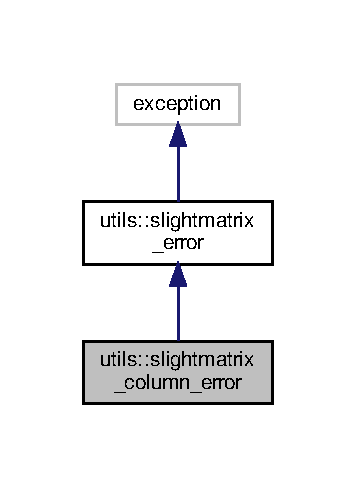
\includegraphics[width=171pt]{classutils_1_1slightmatrix__column__error__inherit__graph}
\end{center}
\end{figure}


Collaboration diagram for utils\+:\+:slightmatrix\+\_\+column\+\_\+error\+:
\nopagebreak
\begin{figure}[H]
\begin{center}
\leavevmode
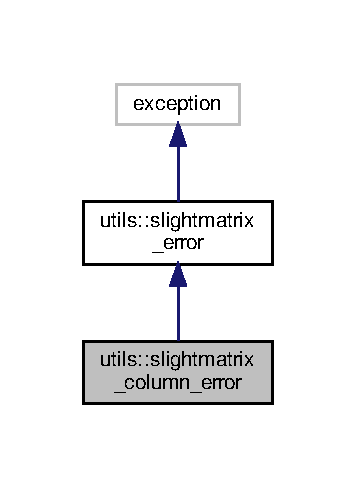
\includegraphics[width=171pt]{classutils_1_1slightmatrix__column__error__coll__graph}
\end{center}
\end{figure}


\subsection{Detailed Description}
Exception inheriting from \hyperlink{classutils_1_1slightmatrix__error}{slightmatrix\+\_\+error}. It is thrown when\+:
\begin{DoxyItemize}
\item method is called with invalid or out-\/of-\/range column count or index. 
\end{DoxyItemize}

The documentation for this class was generated from the following file\+:\begin{DoxyCompactItemize}
\item 
/home/hsg/\+Documents/projects/slightcsv/src/slightmatrix.\+hpp\end{DoxyCompactItemize}

\hypertarget{classutils_1_1slightmatrix__error}{}\section{utils\+:\+:slightmatrix\+\_\+error Class Reference}
\label{classutils_1_1slightmatrix__error}\index{utils\+::slightmatrix\+\_\+error@{utils\+::slightmatrix\+\_\+error}}


Base exception of the class (never gets thrown). Inheriting from std\+::exception.  




{\ttfamily \#include $<$slightmatrix.\+hpp$>$}



Inheritance diagram for utils\+:\+:slightmatrix\+\_\+error\+:
\nopagebreak
\begin{figure}[H]
\begin{center}
\leavevmode
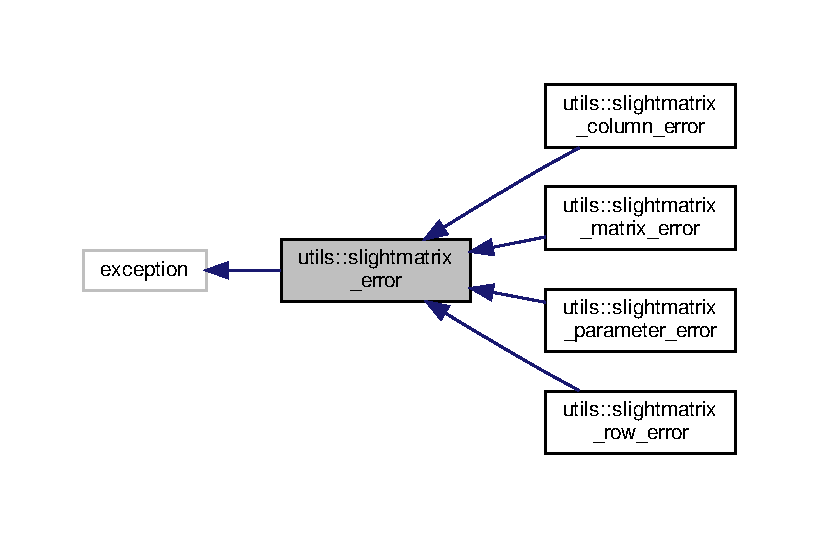
\includegraphics[width=350pt]{classutils_1_1slightmatrix__error__inherit__graph}
\end{center}
\end{figure}


Collaboration diagram for utils\+:\+:slightmatrix\+\_\+error\+:
\nopagebreak
\begin{figure}[H]
\begin{center}
\leavevmode
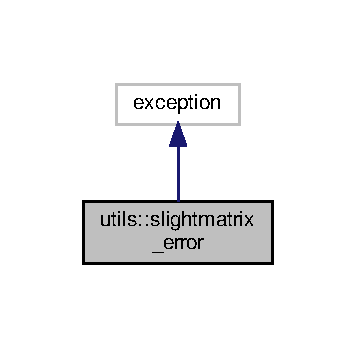
\includegraphics[width=171pt]{classutils_1_1slightmatrix__error__coll__graph}
\end{center}
\end{figure}


\subsection{Detailed Description}
Base exception of the class (never gets thrown). Inheriting from std\+::exception. 

The documentation for this class was generated from the following file\+:\begin{DoxyCompactItemize}
\item 
/home/hsg/\+Documents/projects/slightcsv/src/slightmatrix.\+hpp\end{DoxyCompactItemize}

\hypertarget{classutils_1_1slightmatrix__matrix__error}{}\section{utils\+:\+:slightmatrix\+\_\+matrix\+\_\+error Class Reference}
\label{classutils_1_1slightmatrix__matrix__error}\index{utils\+::slightmatrix\+\_\+matrix\+\_\+error@{utils\+::slightmatrix\+\_\+matrix\+\_\+error}}


{\ttfamily \#include $<$slightmatrix.\+hpp$>$}



Inheritance diagram for utils\+:\+:slightmatrix\+\_\+matrix\+\_\+error\+:
\nopagebreak
\begin{figure}[H]
\begin{center}
\leavevmode
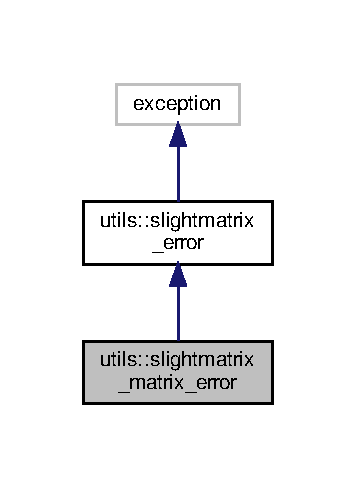
\includegraphics[width=171pt]{classutils_1_1slightmatrix__matrix__error__inherit__graph}
\end{center}
\end{figure}


Collaboration diagram for utils\+:\+:slightmatrix\+\_\+matrix\+\_\+error\+:
\nopagebreak
\begin{figure}[H]
\begin{center}
\leavevmode
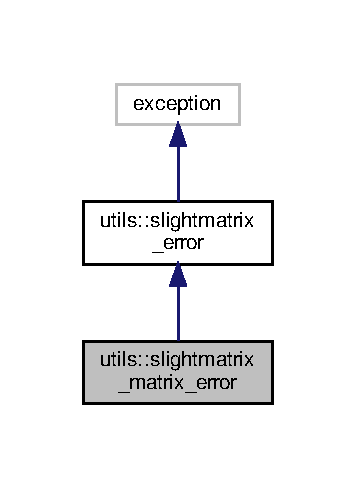
\includegraphics[width=171pt]{classutils_1_1slightmatrix__matrix__error__coll__graph}
\end{center}
\end{figure}


\subsection{Detailed Description}
Exception inheriting from \hyperlink{classutils_1_1slightmatrix__error}{slightmatrix\+\_\+error}. It is thrown when\+:
\begin{DoxyItemize}
\item matrix format is not valid. \begin{DoxySeeAlso}{See also}
validate() 
\end{DoxySeeAlso}

\end{DoxyItemize}

The documentation for this class was generated from the following file\+:\begin{DoxyCompactItemize}
\item 
/home/hsg/\+Documents/projects/slightcsv/src/slightmatrix.\+hpp\end{DoxyCompactItemize}

\hypertarget{classutils_1_1slightmatrix__parameter__error}{}\section{utils\+:\+:slightmatrix\+\_\+parameter\+\_\+error Class Reference}
\label{classutils_1_1slightmatrix__parameter__error}\index{utils\+::slightmatrix\+\_\+parameter\+\_\+error@{utils\+::slightmatrix\+\_\+parameter\+\_\+error}}


{\ttfamily \#include $<$slightmatrix.\+hpp$>$}



Inheritance diagram for utils\+:\+:slightmatrix\+\_\+parameter\+\_\+error\+:\nopagebreak
\begin{figure}[H]
\begin{center}
\leavevmode
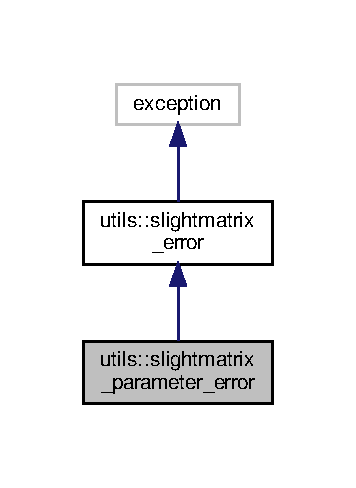
\includegraphics[width=171pt]{classutils_1_1slightmatrix__parameter__error__inherit__graph}
\end{center}
\end{figure}


Collaboration diagram for utils\+:\+:slightmatrix\+\_\+parameter\+\_\+error\+:\nopagebreak
\begin{figure}[H]
\begin{center}
\leavevmode
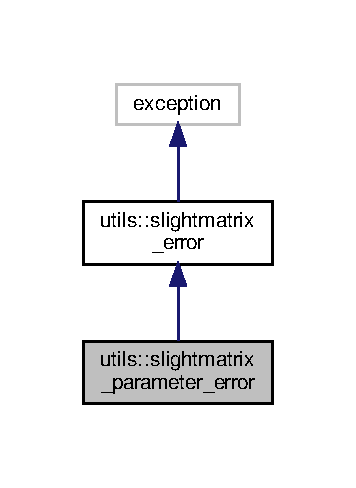
\includegraphics[width=171pt]{classutils_1_1slightmatrix__parameter__error__coll__graph}
\end{center}
\end{figure}


\subsection{Detailed Description}
Exception inheriting from \hyperlink{classutils_1_1slightmatrix__error}{slightmatrix\+\_\+error}. It is thrown when\+:
\begin{DoxyItemize}
\item method is called with zero or empty parameter 
\end{DoxyItemize}

The documentation for this class was generated from the following file\+:\begin{DoxyCompactItemize}
\item 
/home/hsg/\+Documents/projects/slightcsv/src/slightmatrix.\+hpp\end{DoxyCompactItemize}

\hypertarget{classutils_1_1slightmatrix__row__error}{}\section{utils\+:\+:slightmatrix\+\_\+row\+\_\+error Class Reference}
\label{classutils_1_1slightmatrix__row__error}\index{utils\+::slightmatrix\+\_\+row\+\_\+error@{utils\+::slightmatrix\+\_\+row\+\_\+error}}


{\ttfamily \#include $<$slightmatrix.\+hpp$>$}



Inheritance diagram for utils\+:\+:slightmatrix\+\_\+row\+\_\+error\+:\nopagebreak
\begin{figure}[H]
\begin{center}
\leavevmode
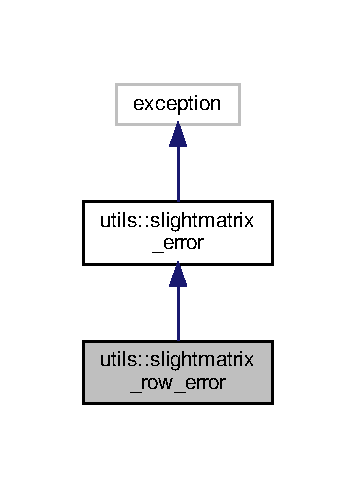
\includegraphics[width=171pt]{classutils_1_1slightmatrix__row__error__inherit__graph}
\end{center}
\end{figure}


Collaboration diagram for utils\+:\+:slightmatrix\+\_\+row\+\_\+error\+:\nopagebreak
\begin{figure}[H]
\begin{center}
\leavevmode
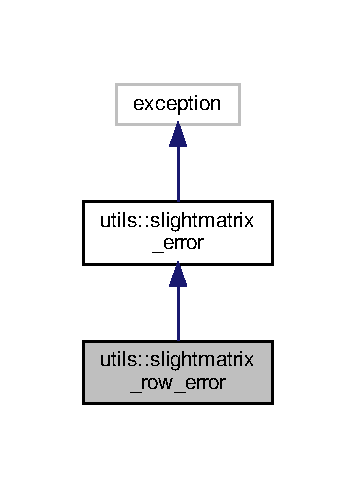
\includegraphics[width=171pt]{classutils_1_1slightmatrix__row__error__coll__graph}
\end{center}
\end{figure}


\subsection{Detailed Description}
Exception inheriting from \hyperlink{classutils_1_1slightmatrix__error}{slightmatrix\+\_\+error}. It is thrown when\+:
\begin{DoxyItemize}
\item method is called with invalid or out-\/of-\/range row count or index. 
\end{DoxyItemize}

The documentation for this class was generated from the following file\+:\begin{DoxyCompactItemize}
\item 
/home/hsg/\+Documents/projects/slightcsv/src/slightmatrix.\+hpp\end{DoxyCompactItemize}

%--- End generated contents ---

% Index
\backmatter
\newpage
\phantomsection
\clearemptydoublepage
\addcontentsline{toc}{chapter}{Index}
\printindex

\end{document}
